% =====================================================================
%  Tesina: Redes neuronales difractivas en el visible
%  Compilar:  latexmk -pdf main.tex     (pdflatex + biber)
%  En Overleaf: compilador pdfLaTeX; la bibliografía usa biber automáticamente.
% =====================================================================
\documentclass[letterpaper,fontsize=12pt,twoside=false,listof=totoc,
               bibliography=totoc,headings=normal,parskip=false]{scrbook}

% =====================================================================
%  Preámbulo de la tesina
% =====================================================================
\usepackage[T1]{fontenc}
\usepackage[utf8]{inputenc}
\usepackage[english,spanish.tabla.noshorthands.nodecimaldot.noquoting.lcroman]{babel}
\usepackage{lmodern}
\usepackage[final]{microtype}
\usepackage{csquotes}

% --- Página -----------------------------------------------------------
\usepackage[letterpaper,top=2.5cm,bottom=2.5cm,inner=3cm,outer=2.5cm]{geometry}
\setkomafont{disposition}{\normalcolor\bfseries}
\setkomafont{chapter}{\color{udlap}\bfseries\huge}
\setkomafont{section}{\color{udlaposcuro}\bfseries\Large}
\usepackage{scrlayer-scrpage}
\pagestyle{scrheadings}
\clearpairofpagestyles
\ohead{\headmark}
\ofoot*{\pagemark}
\automark[section]{chapter}

% --- Colores UDLAP ------------------------------------------------------
\usepackage{xcolor}
\definecolor{udlap}{HTML}{F37B20}        % naranja del logo
\definecolor{udlaposcuro}{HTML}{9A4A0E}
\definecolor{udlapclaro}{HTML}{FDEBDD}
\definecolor{gris}{HTML}{6B6B6B}
\definecolor{azulfig}{HTML}{2C6FB7}

% --- Matemáticas y unidades -------------------------------------------
\usepackage{amsmath,amssymb,amsthm,mathtools,bm}
\usepackage{esint}
\usepackage{siunitx}
\sisetup{output-decimal-marker={.},group-separator={\,},per-mode=symbol,
         range-phrase={--},list-final-separator={ y }}
\numberwithin{equation}{chapter}
\newcommand{\dd}{\,\mathrm{d}}
\newcommand{\jj}{\mathrm{j}}
\newcommand{\FT}{\mathcal{F}}
\newcommand{\IFT}{\mathcal{F}^{-1}}
\newcommand{\rect}{\operatorname{rect}}
\newcommand{\sinc}{\operatorname{sinc}}
\newcommand{\Real}{\operatorname{Re}}
\newcommand{\Imag}{\operatorname{Im}}
\newcommand{\Dmin}{D_{\min}}
\newcommand{\flim}{f_{\lim}}
\DeclareMathOperator*{\argmax}{arg\,max}

\theoremstyle{definition}
\newtheorem{definicion}{Definición}[chapter]
\theoremstyle{plain}
\newtheorem{proposicion}{Proposición}[chapter]
\renewcommand{\qedsymbol}{$\blacksquare$}

% --- Figuras, tablas, diagramas ---------------------------------------
\usepackage{graphicx}
\graphicspath{{figuras/}}
\usepackage{booktabs,multirow,array,tabularx}
\usepackage[font=small,labelfont={bf,color=udlaposcuro},format=hang]{caption}
\usepackage{subcaption}
\usepackage{tikz}
\usetikzlibrary{calc,arrows.meta,decorations.pathreplacing,decorations.pathmorphing,
                patterns,positioning,shapes.geometric,3d,fit,backgrounds}
\usepackage{tikz-3dplot}
\usepackage{pgfplots}
\pgfplotsset{compat=1.18}
\usepgfplotslibrary{fillbetween}

% --- Algoritmos y código -----------------------------------------------
\usepackage{algorithm}
\usepackage{algpseudocode}
\floatname{algorithm}{Algoritmo}
\renewcommand{\listalgorithmname}{Lista de algoritmos}
\algrenewcommand\algorithmicrequire{\textbf{Entrada:}}
\algrenewcommand\algorithmicensure{\textbf{Salida:}}
\usepackage{listings}
\lstset{basicstyle=\ttfamily\footnotesize,breaklines=true,frame=single,
        rulecolor=\color{gris},keywordstyle=\color{udlaposcuro}\bfseries,
        commentstyle=\color{gris}\itshape,numbers=left,numberstyle=\tiny\color{gris},
        literate={á}{{\'a}}1 {é}{{\'e}}1 {í}{{\'i}}1 {ó}{{\'o}}1 {ú}{{\'u}}1 {ñ}{{\~n}}1}

% --- Cajas ---------------------------------------------------------------
\usepackage[most]{tcolorbox}
% Recuadro para resultados clave
\newtcolorbox{resultado}[1]{colback=white,colframe=udlaposcuro,fonttitle=\bfseries,
  title={#1},breakable}
% Recuadro para cálculos numéricos detallados
\newtcolorbox{calculo}[1][]{colback=gray!6,colframe=gray!60,fonttitle=\bfseries\small,
  title={Cálculo: #1},fontupper=\small,breakable}

% --- Bibliografía APA 7 -------------------------------------------------
\usepackage[style=apa,backend=biber]{biblatex}
\addbibresource{referencias.bib}

% --- Enlaces (al final) -------------------------------------------------
\usepackage[hidelinks,pdfusetitle]{hyperref}
\usepackage[spanish,noabbrev]{cleveref}
\crefname{equation}{la ecuación}{las ecuaciones}
\Crefname{equation}{La ecuación}{Las ecuaciones}
\crefname{figure}{la figura}{las figuras}
\Crefname{figure}{La figura}{Las figuras}
\crefname{table}{la tabla}{las tablas}
\Crefname{table}{La tabla}{Las tablas}
\crefname{chapter}{capítulo}{capítulos}
\Crefname{chapter}{Capítulo}{Capítulos}
\crefname{section}{sección}{secciones}
\Crefname{section}{Sección}{Secciones}
\crefname{subsection}{sección}{secciones}
\crefname{appendix}{apéndice}{apéndices}
\crefname{algorithm}{el algoritmo}{los algoritmos}
\Crefname{algorithm}{El algoritmo}{Los algoritmos}
\crefname{proposicion}{la proposición}{las proposiciones}
\Crefname{proposicion}{La proposición}{Las proposiciones}

% =====================================================================
%  DATOS DE LA PORTADA
% =====================================================================
\newcommand{\Titulo}{Redes neuronales difractivas en el visible}
\newcommand{\Subtitulo}{Fundamentos de difracción escalar, criterio de conectividad\\
  y reproducción numérica de \textcite{chen2021}}
\newcommand{\Autor}{Alonso Hernández Hernández y Ángel Gabriel Munguía Velázquez}
\newcommand{\Curso}{Óptica (5.\textsuperscript{o} Semestre)}
\newcommand{\Profesor}{Dr.\ Wanderson Maia Pimienta}
\newcommand{\Departamento}{Actuaría, Física y Matemáticas}
\newcommand{\Escuela}{Ciencias}
\newcommand{\Lugar}{San Andrés Cholula, Puebla}
\newcommand{\Fecha}{2026}


\begin{document}

\frontmatter
% =====================================================================
%  Portada UDLAP. Inspirada en la plantilla original: líneas geométricas
%  finas, bloque de título a la izquierda y datos abajo; aquí todo se dibuja
%  con TikZ (sin imagen de fondo) en el naranja institucional.
% =====================================================================
\begin{titlepage}
\pdfbookmark[0]{Portada}{portada}
\sffamily
\begin{tikzpicture}[remember picture,overlay]
  \coordinate (NW) at (current page.north west);
  \coordinate (SE) at (current page.south east);
  % --- polígono principal (equivalente al marco de la plantilla)
  \draw[udlap!55,line width=0.5pt]
    ($(NW)+(1.2,-3.6)$) -- ($(NW)+(18.6,-2.6)$) -- ($(NW)+(17.2,-23.6)$)
    -- ($(NW)+(1.2,-22.4)$) -- cycle;
  % --- facetas de la derecha
  \draw[udlap!40,line width=0.4pt]
    ($(NW)+(18.6,-2.6)$) -- ($(NW)+(21.6,-0.6)$)
    ($(NW)+(18.6,-2.6)$) -- ($(NW)+(21.6,-7.2)$)
    ($(NW)+(18.3,-7.1)$) -- ($(NW)+(21.6,-8.4)$)
    ($(NW)+(18.3,-7.1)$) -- ($(NW)+(21.6,-12.6)$)
    ($(NW)+(17.9,-13.2)$) -- ($(NW)+(21.6,-12.6)$)
    ($(NW)+(17.6,-16.8)$) -- ($(NW)+(21.6,-18.2)$)
    ($(NW)+(17.2,-23.6)$) -- ($(NW)+(21.6,-18.2)$)
    ($(NW)+(17.2,-23.6)$) -- ($(NW)+(21.6,-27.2)$);
  % --- franja inferior
  \fill[udlap] ($(current page.south west)+(0,0)$) rectangle ($(SE)+(0,0.55)$);
  % --- ondas de difracción sutiles (motivo del tema)
  \foreach \r in {1,...,9}{
    \draw[udlap!18,line width=0.6pt] ($(NW)+(1.2,-22.4)$) ++(0:\r*0.55) arc (0:62:\r*0.55);
  }
  % --- logo
  \node[anchor=north west,inner sep=0pt] at ($(NW)+(1.6,-0.7)$)
    {
\includegraphics[width=2.6cm]{logo_udlap.png}};
  \node[anchor=west,text width=9cm,align=left,inner sep=0pt] at ($(NW)+(4.6,-2.0)$)
    {\fontsize{13}{15}\selectfont\bfseries\color{udlaposcuro}Universidad de las Américas Puebla\\[2pt]
     \fontsize{10}{12}\selectfont\mdseries\color{gris}Escuela de \Escuela\\
     Departamento de \Departamento};
  % --- tipo de trabajo, título y subtítulo
  \node[anchor=north west,inner sep=0pt,text width=14.2cm,align=left]
    at ($(NW)+(2.6,-6.4)$) {%
      {\fontsize{20}{26}\selectfont\color{udlap} Tesina\par}
      \vspace{30pt}
      {\fontsize{22}{27}\selectfont\bfseries \Titulo\par}
      \vspace{12pt}
      {\color{udlap}\rule{3.2cm}{2pt}\par}
      \vspace{12pt}
      {\fontsize{13}{17}\selectfont\mdseries\color{gris} \Subtitulo\par}
  };
  % --- autor, curso, profesor
  \node[anchor=north west,inner sep=0pt,text width=14cm,align=left]
    at ($(NW)+(2.6,-17.0)$) {%
      \fontsize{12}{16}\selectfont
      Presentan: \textbf{\Autor}\par
      \vspace{26pt}
      \fontsize{10.5}{14}\selectfont
      \begin{tabular}{@{}p{3.3cm}@{}p{10cm}@{}}
        Curso:    & \Curso \\[6pt]
        Profesor: & \Profesor \\[6pt]
        Lugar y fecha: & \Lugar, \Fecha
      \end{tabular}
  };
\end{tikzpicture}
\end{titlepage}

% =====================================================================
%  Páginas preliminares
% =====================================================================
\chapter*{Resumen}
\addcontentsline{toc}{chapter}{Resumen}

Las redes neuronales difractivas profundas (D\textsuperscript{2}NN) realizan una tarea de
clasificación únicamente con luz coherente que atraviesa una pila de máscaras de fase
separadas por propagación libre. En este trabajo se reproduce numéricamente el diseño de
\textcite{chen2021}, que lleva este concepto de los terahertz al visible
($\lambda=\SI{632.8}{nm}$), y se deducen paso a paso las ecuaciones que el artículo
presenta sin demostración: el espectro angular a partir de la ecuación de Helmholtz, el
semiángulo de difracción de una neurona y el criterio de conectividad entre capas.
Además, se calcula de forma explícita el gradiente mediante cálculo de Wirtinger y se
muestra que corresponde a retropropagar la señal de error en sentido inverso. Se demuestra que
el criterio de conectividad coincide exactamente con la condición de muestreo
del método de espectro angular de banda limitada, y que en el régimen paraxial su variable
relevante es el número de Fresnel neuronal $N_{F,n}$. La simulación reproduce los casos de
prueba reducidos (\SIrange{89}{91}{\percent}), identifica dos inconsistencias en el artículo y
demuestra mediante barridos sistemáticos en GPU ($L\in\{1,3,5,8\}$) que el criterio es unas
diez veces más estricto de lo necesario porque la conectividad se acumula en $L+1$ etapas.
Finalmente, el entrenamiento en GPU del sistema completo de $1000\times1000$ neuronas y
11 clases alcanza \SI{90.63}{\percent} en prueba (\SI{90.24}{\percent} en dígitos y
\SI{94.50}{\percent} en clase~X), y se cuantifican las tolerancias de fabricación en ocho
niveles de fase, desalineación lateral y separación axial.

\medskip\noindent\textbf{Palabras clave:} difracción escalar, espectro angular, redes
neuronales difractivas, computación óptica, muestreo.

\begin{otherlanguage}{english}
\chapter*{Abstract}
\addcontentsline{toc}{chapter}{Abstract}
Diffractive deep neural networks (D\textsuperscript{2}NNs) perform classification using only
coherent light propagating through a stack of phase masks. This work numerically
reproduces the visible-light design of \textcite{chen2021} at $\lambda=\SI{632.8}{nm}$ and
derives, step by step, the equations that the original article states without proof: the
angular spectrum from the Helmholtz equation, the diffraction half-angle of a neuron, and the
inter-layer connectivity criterion. The training gradient is derived via Wirtinger calculus
and shown to correspond to back-propagating the error field. The connectivity criterion is
proven to coincide with the sampling condition of the band-limited angular spectrum method,
and in the paraxial regime its governing parameter is the single-neuron Fresnel number
$N_{F,n}$. Numerical simulations reproduce the reduced benchmark cases (89--91\,\%), identify
two inconsistencies in the paper, and show through GPU sweeps across $L\in\{1,3,5,8\}$ layers
that the criterion is roughly ten times stricter than necessary due to cumulative diffractive
mixing across $L+1$ stages. Training the full $1000\times1000$-neuron, 11-class visible-light
system achieves 90.63\,\% test accuracy (90.24\,\% on digits 0--9 and 94.50\,\% on altered or
occluded class-X inputs), and fabrication tolerances are quantified for phase quantization,
lateral misalignment, and axial spacing.

\medskip\noindent\textbf{Keywords:} scalar diffraction, angular spectrum, diffractive neural
networks, optical computing, sampling.
\end{otherlanguage}

\tableofcontents
\listoffigures
\listoftables

\chapter*{Lista de símbolos}
\addcontentsline{toc}{chapter}{Lista de símbolos}
\begin{center}
\renewcommand{\arraystretch}{1.25}
\begin{tabularx}{\textwidth}{@{}l X l@{}}
\toprule
Símbolo & Significado & Valor en el sistema del artículo \\
\midrule
$\lambda$ & Longitud de onda en el vacío & \SI{632.8}{nm} (He--Ne)\\
$k$ & Número de onda, $2\pi/\lambda$ & \SI{9.93e6}{m^{-1}}\\
$U(x,y,z)$ & Amplitud compleja escalar del campo & --- \\
$u,\,v$ & Frecuencias espaciales en $x$ y $y$ & --- \\
$\alpha,\beta,\gamma$ & Ángulos del vector de onda con los ejes $x,y,z$ & --- \\
$H(u,v)$ & Función de transferencia de la propagación libre & --- \\
$d_f$ & Tamaño (lado) de una neurona & \SI{4}{\micro m}\\
$\sqrt N$ & Neuronas por lado de una capa & \num{1000}\\
$w$ & Lado de una capa, $w=\sqrt N\,d_f$ & \SI{4}{mm}\\
$D$ & Distancia entre capas consecutivas & \SI{\approx 5}{cm}\\
$L$ & Número de capas difractivas & 5\\
$\Phi^l_i$ & Fase de la neurona $i$ de la capa $l$ & $[0,\pi]$\\
$t^l$ & Transmitancia compleja de la capa $l$, $e^{\jj\Phi^l}$ & --- \\
$\varphi_{\max}$ & Semiángulo máximo de difracción de una neurona & \ang{4.54}\\
$\Dmin$ & Distancia mínima para conectividad total (Ec.~9 del artículo) & \SI{50.4}{mm}\\
$\Delta x$ & Paso de la malla numérica (aquí $\Delta x=d_f$) & \SI{4}{\micro m}\\
$N_p$ & Muestras por lado de la malla con relleno, $N_p=2\sqrt N$ & \num{2000}\\
$\Delta u$ & Paso en frecuencia, $1/(N_p\Delta x)$ & \SI{125}{m^{-1}}\\
$z_c$ & Distancia crítica del espectro angular sin límite de banda & \SI{50.6}{mm}\\
$\flim$ & Frecuencia límite del espectro angular de banda limitada & --- \\
$N_F$ & Número de Fresnel & --- \\
$E_k$ & Energía recogida por el detector $k$ & --- \\
$\Delta n$ & Diferencia de índice entre sustrato y aire & 0.457 (SiO$_2$)\\
\bottomrule
\end{tabularx}
\end{center}


\mainmatter
% =====================================================================
\chapter{Introducción}\label{cap:intro}
% =====================================================================

\section{Motivación y antecedentes}

En el curso de Óptica, la difracción suele presentarse primero a través de sus límites
clásicos —la difracción de campo lejano o de Fraunhofer, donde la propagación libre realiza una
transformada de Fourier espacial exacta, y la difracción de campo cercano o de Fresnel,
gobernada por el principio de Huygens--Fresnel— junto con las herramientas de la óptica de
Fourier y el filtrado espacial en el plano de frecuencias \parencite{goodman2005}. Sin embargo,
esos mismos fenómenos ondulatorios convierten al espacio libre y a los elementos difractivos en
procesadores analógicos masivamente paralelos: al propagarse entre planos modulados, un frente
de onda coherente ejecuta combinaciones lineales complejas a la velocidad de la luz y sin
consumo energético adicional al de la fuente de iluminación.

Mientras que el aprendizaje profundo convencional se ejecuta en procesadores electrónicos cuyo
costo energético y latencia crecen rápidamente con la dimensión de las matrices de pesos,
\textcite{lin2018} propusieron aprovechar la propagación difractiva en una \emph{red neuronal
difractiva profunda} (D\textsuperscript{2}NN): una pila de placas cuya variación local de
espesor impone retardos de fase independientes a la onda incidente. Entrenada numéricamente
en computadora mediante retropropagación y fabricada luego como objeto físico pasivo, la red
clasifica dígitos escritos a mano únicamente mediante interferencia y difracción.

Esa primera demostración operó en la banda de los terahertz ($\lambda\approx\SI{0.75}{mm}$),
donde neuronas de cientos de micrómetros se imprimen en 3D con facilidad. Estudios posteriores
profundizaron en la capacidad de representación de estas arquitecturas, su sensibilidad al
número de capas y las ventajas de integrarlas con etapas electrónicas de detección
\parencite{mengu2020}, confirmando que la profundidad óptica aporta grados de libertad que una
sola máscara no alcanza. No obstante, trasladar el esquema al espectro visible ofrece ventajas
decisivas: reduce el tamaño transversal del sistema en tres órdenes de magnitud y habilita
fuentes láser compactas y detectores CMOS convencionales. A cambio, exige fabricar neuronas de
escala micrométrica por fotolitografía y plantea una restricción física fundamental sobre el
espaciamiento entre planos: al disminuir $d_f$ o acortar $\lambda$, el cono de difracción de
cada píxel cambia de abertura y condiciona si las capas logran mezclarse entre sí.
\textcite{chen2021} abordan precisamente este régimen en el visible con un láser de He--Ne
($\lambda=\SI{632.8}{nm}$), proponen un criterio cuantitativo de conectividad entre capas y
demuestran experimentalmente un clasificador pasivo de cinco capas en sílice fundida.

\section{Planteamiento del problema}

El artículo de \textcite{chen2021} presenta su modelo físico (sus ecuaciones~1 a~5) y su
criterio de conectividad (ecuaciones~6 a~9) sin deducirlos, y valida el criterio con sólo
cuatro configuraciones numéricas. Tampoco describe cómo se discretiza la propagación ni
cómo se calcula el gradiente durante el entrenamiento. Este trabajo se propone llenar esos
huecos desde la teoría de la difracción escalar y comprobar los resultados mediante una
reproducción numérica independiente.

\section{Objetivos}

\paragraph{Objetivo general.} Deducir, justificar y reproducir numéricamente el modelo de
una D\textsuperscript{2}NN de solo fase en el visible propuesto por \textcite{chen2021}.

\paragraph{Objetivos específicos.}
\begin{enumerate}
  \item Deducir la función de transferencia del espacio libre (espectro angular) a partir de
        la ecuación de Helmholtz, y relacionarla con la integral de Rayleigh--Sommerfeld.
  \item Justificar el semiángulo de difracción $\varphi_{\max}=\arcsin[\lambda/(2d_f)]$ y
        deducir el criterio de conectividad entre capas.
  \item Obtener explícitamente el gradiente de la función de pérdida respecto a las fases.
  \item Analizar el muestreo numérico de la propagación y validar el propagador contra
        soluciones analíticas.
  \item Reproducir la Fig.~6 del artículo y explorar el criterio de conectividad con un
        barrido de la distancia entre capas.
  \item Estimar las tolerancias de fabricación del sistema.
\end{enumerate}

\section{Contribuciones}\label{sec:contribuciones}

Además de la reproducción, este trabajo aporta los siguientes elementos que no aparecen en el
artículo original:
\begin{enumerate}
  \item La deducción completa de las ecuaciones del modelo, desde la ecuación de Helmholtz
        hasta el criterio de conectividad (\cref{cap:difraccion,cap:modelo,cap:conectividad}).
  \item La justificación del factor~2 en $\varphi_{\max}=\arcsin[\lambda/(2d_f)]$ mediante el
        teorema de muestreo (\cref{sec:neurona}).
  \item El cálculo del gradiente con cálculo de Wirtinger y su interpretación como una onda
        de error que viaja en sentido inverso (\cref{sec:gradiente}).
  \item La demostración de que el criterio de conectividad coincide con la condición de
        muestreo del espectro angular de banda limitada (\cref{prop:identidad}), y de que su
        variable relevante es el número de Fresnel de una neurona (\cref{sec:fresnel-neurona}).
  \item Un barrido de la distancia entre capas que muestra que el criterio es unas diez veces
        más estricto de lo necesario (\cref{sec:barrido}).
  \item La identificación de dos inconsistencias en la Fig.~6 del artículo
        (\cref{sec:inconsistencias}) y un análisis de tolerancias de fabricación
        (\cref{sec:fabricacion}).
\end{enumerate}

\section{Organización del documento}

El \cref{cap:difraccion} desarrolla la teoría de la difracción escalar necesaria. El
\cref{cap:modelo} construye el modelo de la red y deduce su gradiente. El
\cref{cap:conectividad} analiza la conectividad entre capas. El \cref{cap:numerico} describe
la discretización y valida el propagador. El \cref{cap:resultados} presenta los resultados y
el \cref{cap:conclusiones}, las conclusiones. Los apéndices contienen la deducción de la
integral de Rayleigh--Sommerfeld y detalles de implementación.

% =====================================================================
\chapter{Fundamentos de difracción escalar}\label{cap:difraccion}
% =====================================================================

Este capítulo construye, desde las ecuaciones de Maxwell, la herramienta que usa todo el
modelo: la propagación de un campo escalar entre dos planos paralelos. Se sigue la
exposición de \textcite[caps.~3--4]{goodman2005}, con la notación de \textcite{chen2021}.

\section{De las ecuaciones de Maxwell a la ecuación de Helmholtz}\label{sec:helmholtz}

En un medio lineal, isótropo, homogéneo y no dispersivo, sin cargas ni corrientes libres,
cada componente cartesiana del campo eléctrico satisface la ecuación de onda
\parencite[sec.~3.2]{goodman2005}
\begin{equation}
  \nabla^2 \mathcal{U}(\bm r,t)-\frac{n^2}{c^2}\frac{\partial^2 \mathcal{U}(\bm r,t)}{\partial t^2}=0,
  \label{eq:onda}
\end{equation}
donde $n$ es el índice de refracción y $c$ la velocidad de la luz en el vacío. Para luz
monocromática escribimos
\begin{equation}
  \mathcal{U}(\bm r,t)=\Real\!\left\{U(\bm r)\,e^{-\jj\omega t}\right\},
  \label{eq:fasor}
\end{equation}
donde $U(\bm r)$ es la \emph{amplitud compleja}. Al sustituir \eqref{eq:fasor} en
\eqref{eq:onda}, la derivada temporal produce un factor $(-\jj\omega)^2=-\omega^2$, y se obtiene
la \emph{ecuación de Helmholtz}
\begin{equation}
  \left(\nabla^2+k^2\right)U(\bm r)=0,\qquad k=\frac{n\omega}{c}=\frac{2\pi n}{\lambda}.
  \label{eq:helmholtz}
\end{equation}
En aire ($n\approx1$) y con $\lambda=\SI{632.8}{nm}$, el número de onda vale
$k=2\pi/\lambda=\SI{9.93e6}{m^{-1}}$.

\paragraph{Convención de signos.} Con la dependencia temporal $e^{-\jj\omega t}$ de
\eqref{eq:fasor}, una onda plana que se propaga hacia $+z$ tiene la forma $e^{+\jj kz}$, la
misma convención empleada por \textcite{chen2021} en su Ec.~2.

\paragraph{Validez de la aproximación escalar.} Tratar cada componente por separado ignora
el acoplamiento entre componentes que introducen los bordes de las aperturas. Ese
acoplamiento es despreciable si las estructuras son mucho mayores que $\lambda$ y el campo se
observa lejos de ellas \parencite[sec.~3.2]{goodman2005}. En el sistema del artículo
$d_f=\SI{4}{\micro m}\approx6.3\lambda$, de modo que la aproximación es razonable. En cambio, el
caso~1 de su Fig.~6 ($d_f=0.53\lambda$) queda fuera de su rango de validez; volveremos a
esto en el \cref{cap:conclusiones}.

\section{Principio de Huygens--Fresnel e integral de Rayleigh--Sommerfeld}\label{sec:rs}

Supongamos que conocemos el campo $U(x',y',0)$ en el plano $z=0$ y que todas las fuentes
están en $z<0$. Aplicando el teorema de Green con una función de Green que se anula en el
plano $z=0$ (\cref{ap:rs}) se obtiene la \emph{integral de Rayleigh--Sommerfeld de primera
especie} \parencite[sec.~3.5]{goodman2005}:
\begin{equation}
  U(x,y,z)=\iint_{-\infty}^{\infty} U(x',y',0)\;h(x-x',y-y',z)\dd x'\dd y',
  \label{eq:rs}
\end{equation}
con la \emph{respuesta al impulso}
\begin{equation}
  h(x,y,z)=\frac{z}{2\pi r^2}\left(\frac{1}{r}-\jj k\right)e^{\jj kr},
  \qquad r=\sqrt{x^2+y^2+z^2}.
  \label{eq:h-rs}
\end{equation}
Cuando $r\gg\lambda$ domina el término $-\jj k$, y como $-\jj k/(2\pi)=1/(\jj\lambda)$,
\begin{equation}
  h(x,y,z)\approx\frac{1}{\jj\lambda}\,\frac{z}{r}\,\frac{e^{\jj kr}}{r}.
  \label{eq:huygens}
\end{equation}
\Cref{eq:huygens} expresa matemáticamente el principio de Huygens--Fresnel
(\cref{fig:huygens}): cada punto del plano $z=0$ emite una onda esférica secundaria
$e^{\jj kr}/r$, adelantada un cuarto de periodo (factor $1/\jj$), con amplitud proporcional a
$1/\lambda$ y modulada por el factor de oblicuidad $z/r=\cos\theta$. En una D\textsuperscript{2}NN
estas ondas secundarias son precisamente las ``conexiones'' entre una neurona y las de la
capa siguiente.

\begin{figure}[htb]
\centering
\begin{tikzpicture}[scale=1.0,>={Stealth[length=2.2mm]}]
  % plano de la apertura
  \fill[gray!15] (0,-2.5) rectangle (0.18,2.5);
  \draw[thick] (0.18,-2.5) -- (0.18,2.5);
  \node[above] at (0.05,2.7) {\small plano $z=0$};
  % frente incidente
  \foreach \x in {-2.4,-1.8,-1.2} \draw[azulfig!70,thick] (\x,-2.1) -- (\x,2.1);
  \draw[->,azulfig,thick] (-2.6,0) -- (-0.6,0);
  \node[azulfig,above,font=\small] at (-1.8,2.28) {onda incidente};
  % fuentes secundarias y ondas esféricas
  \foreach \y in {-1.4,-0.7,0,0.7,1.4}{
     \fill[udlap] (0.18,\y) circle (1.6pt);
     \foreach \r in {0.45,0.9,1.35}
        \draw[udlap!70] ($(0.18,\y)+(-80:\r)$) arc (-80:80:\r);
  }
  % envolvente
  \draw[udlaposcuro,very thick,dashed] (1.55,-2.1) -- (1.55,2.1);
  \node[udlaposcuro,right,align=left] at (1.70,1.85) {\small envolvente:\\ \small nuevo frente};
  % punto de observación
  \coordinate (P) at (5.6,0.9);
  \fill (P) circle (1.8pt) node[right] {\small $P(x,y,z)$};
  \draw[->,gray] (0.18,-0.7) -- (P) node[midway,below,sloped] {\small $r$};
  \draw[gray,dashed] (0.18,-0.7) -- (5.6,-0.7);
  \draw[gray] ($(0.18,-0.7)+(1.4,0)$) arc (0:{atan(1.6/5.42)}:1.4);
  \node[gray] at (1.95,-0.45) {\small $\theta$};
  \draw[->] (0.18,-2.8) -- (6.2,-2.8) node[right] {$z$};
\end{tikzpicture}
\caption[Principio de Huygens--Fresnel]{Principio de Huygens--Fresnel. Cada punto del
plano $z=0$ actúa como fuente de una onda esférica secundaria; el campo en $P$ es la
superposición de todas ellas ponderada por el factor de oblicuidad $\cos\theta=z/r$
(\cref{eq:huygens}).}
\label{fig:huygens}
\end{figure}

\section{Espectro angular de ondas planas}\label{sec:espectro-angular}

La integral \eqref{eq:rs} es una convolución bidimensional, lo que sugiere trabajar en el
dominio de Fourier. Escribimos el campo en cualquier plano $z$ como una superposición de
ondas planas \parencite[sec.~3.10]{goodman2005}:
\begin{equation}
  \begin{aligned}
  U(x,y,z)&=\iint_{-\infty}^{\infty}A(u,v;z)\,e^{\jj2\pi(ux+vy)}\dd u\dd v,\\
  A(u,v;z)&=\iint_{-\infty}^{\infty}U(x,y,z)\,e^{-\jj2\pi(ux+vy)}\dd x\dd y,
  \end{aligned}
  \label{eq:espectro}
\end{equation}
donde $u$ y $v$ son \emph{frecuencias espaciales} (en \si{m^{-1}}) y $A(u,v;z)$ es el
\emph{espectro angular} del campo en el plano $z$.

\subsection{Significado físico de las frecuencias espaciales}

Una onda plana de amplitud unitaria cuyo vector de onda forma los ángulos $\alpha$, $\beta$
y $\gamma$ con los ejes $x$, $y$ y $z$ (\cref{fig:cosenos}) es
\begin{equation}
  e^{\jj\bm k\cdot\bm r}=\exp\!\left[\jj k\left(x\cos\alpha+y\cos\beta+z\cos\gamma\right)\right],
  \qquad \cos^2\alpha+\cos^2\beta+\cos^2\gamma=1 .
  \label{eq:onda-plana}
\end{equation}
En el plano $z=0$ esta onda vale $\exp[\jj2\pi(x\cos\alpha/\lambda+y\cos\beta/\lambda)]$.
Comparando con el núcleo de \eqref{eq:espectro} se identifica
\begin{equation}
  u=\frac{\cos\alpha}{\lambda},\qquad v=\frac{\cos\beta}{\lambda},\qquad
  \cos\gamma=\sqrt{1-\lambda^2\left(u^2+v^2\right)} .
  \label{eq:cosenos}
\end{equation}
Así, cada par $(u,v)$ corresponde a una onda plana que viaja en una dirección concreta: las
frecuencias espaciales altas son ondas muy inclinadas. Esta es la definición de $u$ y $v$
que usa \textcite{chen2021} entre sus Ecs.~2 y~3.

\begin{figure}[htb]
\centering
\tdplotsetmaincoords{70}{125}
\begin{tikzpicture}[tdplot_main_coords,scale=3.2,>={Stealth[length=2mm]}]
  \draw[->] (0,0,0) -- (1.5,0,0) node[anchor=north east] {$x$};
  \draw[->] (0,0,0) -- (0,1.5,0) node[anchor=north west] {$y$};
  \draw[->] (0,0,0) -- (0,0,1.45) node[anchor=south] {$z$};
  \coordinate (K) at (0.85,0.70,0.95);
  \draw[->,very thick,udlap] (0,0,0) -- (K) node[anchor=south west] {$\bm k$};
  \draw[dashed,gray] (K) -- (0.85,0.70,0) -- (0,0,0);
  \draw[dashed,gray] (0.85,0.70,0) -- (0.85,0,0);
  \draw[dashed,gray] (0.85,0.70,0) -- (0,0.70,0);
  % ángulos
  \tdplotdefinepoints(0,0,0)(1,0,0)(0.85,0.70,0.95)
  \tdplotdrawpolytopearc[thick,azulfig]{0.50}{anchor=south east}{$\alpha$}
  \tdplotdefinepoints(0,0,0)(0,1,0)(0.85,0.70,0.95)
  \tdplotdrawpolytopearc[thick,azulfig]{0.52}{anchor=south west}{$\beta$}
  \tdplotdefinepoints(0,0,0)(0,0,1)(0.85,0.70,0.95)
  \tdplotdrawpolytopearc[thick,azulfig]{0.82}{anchor=south}{$\gamma$}
\end{tikzpicture}
\caption[Cosenos directores del vector de onda]{Ángulos del vector de onda $\bm k$ con los
ejes coordenados. La componente de una onda plana con frecuencias espaciales $(u,v)$ viaja
en la dirección dada por \cref{eq:cosenos}.}
\label{fig:cosenos}
\end{figure}

\subsection{Propagación del espectro angular}

Sustituimos la representación \eqref{eq:espectro} en la ecuación de Helmholtz
\eqref{eq:helmholtz}. Las derivadas respecto a $x$ y $y$ actúan sólo sobre la exponencial y
producen $\partial_x^2+\partial_y^2\to-4\pi^2(u^2+v^2)$; por lo tanto, para cada $(u,v)$,
\begin{equation}
  \frac{\dd^2A(u,v;z)}{\dd z^2}+k_z^2\,A(u,v;z)=0,
  \qquad k_z=2\pi\sqrt{\frac{1}{\lambda^2}-u^2-v^2}=k\sqrt{1-\lambda^2(u^2+v^2)} .
  \label{eq:edo}
\end{equation}
\Cref{eq:edo} es la ecuación de un oscilador armónico en la variable $z$. Su solución
general es $A(z)=A_+e^{\jj k_zz}+A_-e^{-\jj k_zz}$. Como todas las fuentes están en $z<0$, sólo
puede haber ondas que se alejan del plano inicial, y se descarta $A_-$. Imponiendo
$A(u,v;0)$ como condición inicial,
\begin{equation}
  A(u,v;z)=A(u,v;0)\,\exp\!\left[\jj kz\sqrt{1-\lambda^2\left(u^2+v^2\right)}\right].
  \label{eq:prop-espectro}
\end{equation}
Con \eqref{eq:cosenos}, el exponente es $\jj kz\cos\gamma$: cada onda plana acumula la fase
correspondiente a recorrer la distancia $z$ en su propia dirección. Ésta es exactamente la
Ec.~2 de \textcite{chen2021}, y su Ec.~3 es la misma expresión escrita con $u$ y $v$.

\subsection{Función de transferencia del espacio libre}

\Cref{eq:prop-espectro} dice que la propagación libre es un \emph{sistema lineal e
invariante ante traslaciones} con función de transferencia
\begin{equation}
  H(u,v;z)=
  \begin{cases}
    \exp\!\left[\jj kz\sqrt{1-\lambda^2(u^2+v^2)}\right], & u^2+v^2\le 1/\lambda^2,\\[6pt]
    \exp\!\left[-2\pi z\sqrt{u^2+v^2-1/\lambda^2}\right], & u^2+v^2> 1/\lambda^2,
  \end{cases}
  \label{eq:H}
\end{equation}
de modo que
\begin{equation}
  \boxed{\;U(x,y,z)=\IFT\Bigl\{\FT\{U(x,y,0)\}\cdot H(u,v;z)\Bigr\}.\;}
  \label{eq:asm}
\end{equation}
La segunda rama de \eqref{eq:H} corresponde a las \emph{ondas evanescentes}: cuando
$u^2+v^2>1/\lambda^2$ la raíz es imaginaria y la onda decae exponencialmente en $z$. Esas
componentes describen detalles del campo menores que $\lambda$ y no llegan a la capa
siguiente. Por el teorema de convolución, $H$ es la transformada de Fourier de la respuesta
al impulso \eqref{eq:h-rs}, de modo que \eqref{eq:asm} y \eqref{eq:rs} son
\emph{exactamente} equivalentes \parencite[sec.~3.10]{goodman2005}.

\paragraph{Observación sobre la notación del artículo.} Las Ecs.~4 y~5 de
\textcite{chen2021} escriben el campo de salida multiplicando $W^{l+1}$ por el factor
$\exp\bigl[\jj kd_l\sqrt{1-\lambda^2(u^2+v^2)}\bigr]$. Tomada literalmente, esa
expresión mezcla una función de $(x,y)$ con una de $(u,v)$; el producto debe hacerse en el
dominio de Fourier, como en \eqref{eq:asm}. En el \cref{cap:modelo} se usa la forma correcta.

\section{Aproximaciones de Fresnel y Fraunhofer}\label{sec:fresnel}

Muchos cursos de óptica resuelven la difracción con las aproximaciones de Fresnel o de
Fraunhofer. Conviene comprobar si son válidas para este sistema, porque de ello depende qué
propagador hay que usar.

\paragraph{Aproximación de Fresnel.} Con $\rho^2=u^2+v^2$ y $s=\lambda^2\rho^2$, el desarrollo
binomial $\sqrt{1-s}=1-\tfrac{s}{2}-\tfrac{s^2}{8}-\dots$ convierte \eqref{eq:H} en
\begin{equation}
  H(u,v;z)=e^{\jj kz}\;
  \underbrace{e^{-\jj\pi\lambda z\rho^2}}_{\text{término de Fresnel}}\;
  \underbrace{e^{-\jj kz\lambda^4\rho^4/8}}_{\text{se desprecia}}\cdots
  \label{eq:fresnel-tf}
\end{equation}
La aproximación de Fresnel conserva sólo los dos primeros factores. Es válida si la fase
del tercero es pequeña:
\begin{equation}
  \frac{kz\lambda^4\rho^4}{8}=\frac{\pi z\lambda^3\rho^4}{4}\ll 1 .
  \label{eq:fresnel-cond}
\end{equation}

\begin{calculo}[¿Es válida la aproximación de Fresnel en el sistema del artículo?]
La malla de neuronas sólo puede representar frecuencias hasta $\rho=1/(2d_f)$ en cada eje
(\cref{sec:neurona}). Sustituyendo $\rho^4=1/(16d_f^4)$ en \eqref{eq:fresnel-cond}:
\[
  \frac{\pi z\lambda^3}{64\,d_f^4}
  =\frac{\pi(\SI{0.05}{m})(\SI{632.8e-9}{m})^3}{64\,(\SI{4e-6}{m})^4}
  =\frac{\pi\,(\num{1.267e-20})}{\num{1.638e-20}}
  \approx\SI{2.4}{rad}.
\]
El término despreciado no es pequeño (en la diagonal, donde $\rho^4$ es cuatro veces
mayor, llega a \SI{9.7}{rad}). \textbf{La aproximación de Fresnel no es válida} para las
componentes más inclinadas; por eso en este trabajo se usa la función de transferencia
exacta \eqref{eq:H}.
\end{calculo}

\paragraph{Aproximación de Fraunhofer.} Exige además $z\gg k a^2/2$, con $a$ la semianchura
de la apertura \parencite[sec.~4.3]{goodman2005}. Para una capa de $w=\SI{4}{mm}$
($a=\SI{2}{mm}$), $ka^2/2=\pi a^2/\lambda\approx\SI{19.9}{m}$, cuatrocientas veces la
separación entre capas. El número de Fresnel de una capa,
$N_F=a^2/(\lambda D)=(\SI{2}{mm})^2/(\SI{632.8}{nm}\times\SI{5}{cm})\approx126$, confirma que el
sistema opera en \emph{campo cercano}: la luz no forma entre capas el patrón de Fraunhofer
de la capa completa.

\section{Difracción de una neurona y el ángulo máximo}\label{sec:neurona}

\textcite{chen2021} afirman, citando a \textcite{lin2018}, que el semiángulo máximo de
difracción de una neurona de tamaño $d_f$ es
\begin{equation}
  \varphi_{\max}=\arcsin\!\left(\frac{\lambda}{2d_f}\right),
  \label{eq:phimax}
\end{equation}
sin justificarlo. Aquí se deduce y se explica el factor~2.

\subsection{Una neurona aislada: la función sinc}

Una neurona aislada es una apertura cuadrada de lado $d_f$: $t(x,y)=\rect(x/d_f)\rect(y/d_f)$.
Su espectro angular es
\begin{equation}
  T(u,v)=d_f^2\,\sinc(d_fu)\,\sinc(d_fv),\qquad \sinc(x)\equiv\frac{\sin(\pi x)}{\pi x},
  \label{eq:sinc}
\end{equation}
y, por \eqref{eq:cosenos}, la intensidad radiada en la dirección $\sin\theta=\lambda u$ es
proporcional a $\sinc^2(d_f\sin\theta/\lambda)$ (\cref{fig:sinc}). El primer cero está en
$d_fu=1$, es decir en $\sin\theta=\lambda/d_f$, \emph{no} en $\lambda/(2d_f)$. En la dirección
$\sin\theta=\lambda/(2d_f)$ la intensidad aún vale $\sinc^2(1/2)=4/\pi^2\approx\SI{40.5}{\percent}$
del máximo.

\begin{figure}[htb]
\centering
\begin{tikzpicture}
\begin{axis}[width=0.86\textwidth,height=3.6cm,
  xlabel={$d_f\,u=d_f\sin\theta/\lambda$}, ylabel={$\sinc^2(d_fu)$},
  xmin=-2.6,xmax=2.6,ymin=0,ymax=1.15,samples=400,domain=-2.6:2.6,
  xtick={-2,-1,-0.5,0,0.5,1,2},
  xticklabels={$-2$,$-1$,$-\tfrac12$,$0$,$\tfrac12$,$1$,$2$},
  axis lines=left,grid=major,grid style={gray!20},
  legend style={at={(0.5,1.04)},anchor=south,legend columns=2,column sep=8pt,font=\footnotesize,draw=none,fill=none}]
  \addplot[name path=f,very thick,udlap] {x==0 ? 1 : (sin(deg(pi*x))/(pi*x))^2};
  \addlegendentry{intensidad radiada por una neurona}
  \path[name path=axis] (axis cs:-0.5,0) -- (axis cs:0.5,0);
  \addplot[udlap!25] fill between[of=f and axis,soft clip={domain=-0.5:0.5}];
  \addlegendentry{banda de Nyquist: \SI{77.4}{\percent} de la energía (1D)}
  \draw[dashed,thick,azulfig] (axis cs:0.5,0) -- (axis cs:0.5,1.02);
  \node[font=\footnotesize,azulfig,anchor=west] at (axis cs:0.54,0.96) {$\sin\varphi_{\max}=\lambda/(2d_f)$};
  \draw[dashed,thick,gray] (axis cs:1,0) -- (axis cs:1,0.52);
  \node[font=\footnotesize,gray,align=left,anchor=west] at (axis cs:1.05,0.44) {primer cero\\$\sin\theta=\lambda/d_f$};
  \draw[dotted,thick] (axis cs:-2.6,0.405) -- (axis cs:0.5,0.405);
  \node[font=\footnotesize,anchor=south west] at (axis cs:-2.55,0.42) {$4/\pi^2\approx0.405$};
\end{axis}
\end{tikzpicture}
\caption[Patrón de difracción de una neurona]{Intensidad radiada por una neurona cuadrada
en función de la frecuencia espacial. El área sombreada es la banda que la malla de
neuronas puede controlar ($|u|\le1/2d_f$); su borde define $\varphi_{\max}$ (\cref{eq:phimax}).}
\label{fig:sinc}
\end{figure}

\subsection{Una capa de neuronas: el teorema de muestreo}

El factor~2 aparece al considerar la capa completa. Una capa de solo fase con neuronas de
lado $d_f$ centradas en $x_i=i\,d_f$ tiene transmitancia
\begin{equation}
  t(x)=\sum_i t_i\,\rect\!\left(\frac{x-x_i}{d_f}\right)
      =\Bigl[\sum_i t_i\,\delta(x-x_i)\Bigr]*\rect\!\left(\frac{x}{d_f}\right),
  \qquad t_i=e^{\jj\Phi_i},
  \label{eq:capa-muestreada}
\end{equation}
(en una dimensión, para simplificar). Por el teorema de convolución, su espectro es el
producto del espectro de la secuencia de muestras, que es \emph{periódico} con periodo
$1/d_f$, por la envolvente $d_f\sinc(d_fu)$. Toda la información que el diseñador controla
(los valores $t_i$) está contenida en un solo periodo, $|u|\le1/(2d_f)$; las réplicas fuera de
esa banda son copias atenuadas por la sinc y no pueden ajustarse de forma independiente.
Ésta es la frecuencia de Nyquist del teorema de muestreo \parencite{shannon1949}.

Por lo tanto, la dirección más inclinada hacia la que la red puede enviar luz \emph{de
manera controlada} cumple $\sin\varphi_{\max}=\lambda u_{\text{Nyquist}}=\lambda/(2d_f)$, que es
\eqref{eq:phimax}. Como muestra \cref{fig:sinc}, esa banda contiene el
$\int_{-1/2}^{1/2}\sinc^2(x)\dd x\approx\SI{77.4}{\percent}$ de la energía radiada por una
neurona en cada dirección (el \SI{59.9}{\percent} en dos dimensiones).

\begin{calculo}[Semiángulo de difracción en el sistema del artículo]
Con $d_f=\SI{4}{\micro m}$ y $\lambda=\SI{632.8}{nm}$:
\[
  \sin\varphi_{\max}=\frac{\num{632.8e-9}}{2\times\num{4e-6}}=\num{0.0791}
  \quad\Rightarrow\quad\varphi_{\max}=\ang{4.54},
  \qquad\tan\varphi_{\max}=\num{0.0793}.
\]
En la demostración en terahertz de \textcite{lin2018} ($\lambda=\SI{0.75}{mm}$,
$d_f=\SI{0.4}{mm}$) el mismo cálculo da $\sin\varphi_{\max}=0.94$, es decir $\varphi_{\max}\approx\ang{70}$.
Mantener ese ángulo en el visible exigiría neuronas de $\approx\SI{330}{nm}$, como señalan
\textcite{chen2021}; de ahí la necesidad de compensar con la distancia entre capas.
\end{calculo}

% =====================================================================
\chapter{Modelo de la red neuronal difractiva}\label{cap:modelo}
% =====================================================================

Con la propagación libre resuelta en el \cref{cap:difraccion}, este capítulo construye el
modelo completo de la red: cómo actúa una capa, cómo se encadenan las capas, cómo se
convierte la luz de salida en una clasificación y cómo se calcula el gradiente necesario
para entrenarla.

\section{Descripción del sistema}\label{sec:sistema}

\Cref{fig:sistema} resume el arreglo de \textcite{chen2021}. Un láser de He--Ne se
expande y filtra espacialmente con dos lentes y un orificio, de modo que una onda plana
ilumina el objeto de entrada: un dígito escrito a mano grabado como máscara binaria de cromo
sobre vidrio. La luz atraviesa cinco capas difractivas de solo fase, separadas por
$D\approx\SI{5}{cm}$, y llega a un plano de salida con once regiones de detección: una por
cada dígito del 0 al 9 y una clase adicional ``X'' para dígitos tapados o alterados. La
clase asignada es la del detector que recibe más energía. \Cref{tab:parametros} reúne los
parámetros.

\begin{figure}[htb]
\centering
\begin{tikzpicture}[x=0.93cm,y=1cm,>={Stealth[length=2mm]},
  capa/.style={fill=udlap!25,draw=udlaposcuro,thick},
  plano/.style={fill=gray!10,draw=gray!70,thick}]
  % haz
  \fill[red!12] (0.9,-0.25) -- (2.3,-0.9) -- (13.0,-0.9) -- (13.0,0.9) -- (2.3,0.9) -- cycle;
  % láser
  \draw[fill=gray!60,rounded corners=2pt] (-0.9,-0.35) rectangle (0.9,0.35);
  \node[font=\scriptsize,white] at (0,0) {He--Ne};
  \node[font=\scriptsize,below] at (0,-0.4) {\SI{632.8}{nm}};
  % lentes y orificio
  \draw[thick,azulfig] (1.6,0) ellipse (0.07 and 0.45);
  \draw[very thick] (1.95,0.5) -- (1.95,0.06) (1.95,-0.06) -- (1.95,-0.5);
  \draw[thick,azulfig] (2.6,0) ellipse (0.12 and 1.05);
  \node[font=\scriptsize,align=center,below] at (2.1,-1.1) {lentes y\\orificio};
  % planos oblicuos
  \newcommand{\placa}[3]{%
    \draw[#3] ($(#1,0)+(-0.25,-1.15)$) -- ($(#1,0)+(0.25,-0.75)$) -- ($(#1,0)+(0.25,1.35)$)
             -- ($(#1,0)+(-0.25,0.95)$) -- cycle;
    \node[font=\scriptsize,below] at ($(#1,0)+(0,-1.2)$) {#2};}
  \placa{3.6}{entrada}{plano}
  \node at (3.6,0.1) {\scriptsize\bfseries 3};
  \foreach \l/\x in {1/5.0,2/6.4,3/7.8,4/9.2,5/10.6} {\placa{\x}{$L_{\l}$}{capa}}
  \placa{12.2}{salida}{plano}
  \foreach \yy in {-0.6,0,0.6} \draw[fill=white,draw=red!70!black] ($(12.2,\yy)+(-0.06,-0.08)$) rectangle ($(12.2,\yy)+(0.1,0.12)$);
  % distancias
  \draw[<->] (5.0,1.65) -- (6.4,1.65) node[midway,above,font=\scriptsize] {$D\approx\SI{5}{cm}$};
  \draw[decorate,decoration={brace,amplitude=4pt,mirror}] (4.75,-1.65) -- (10.85,-1.65)
     node[midway,below=4pt,font=\scriptsize] {5 capas de $1000\times1000$ neuronas de \SI{4}{\micro m}};
  \draw[->,thick] (13.0,0) -- (13.8,0) node[right,font=\scriptsize,align=left] {$\argmax_k E_k$};
\end{tikzpicture}
\caption[Esquema del sistema]{Esquema del clasificador de \textcite{chen2021}. La onda
plana modulada por el dígito atraviesa cinco capas de solo fase; cada detector del plano de
salida integra la intensidad sobre su área.}
\label{fig:sistema}
\end{figure}

\begin{table}[htb]
\centering
\caption{Parámetros del sistema de \textcite{chen2021} y de los casos de su Fig.~6.}
\label{tab:parametros}
\begin{tabular}{@{}lll@{}}
\toprule
Parámetro & Sistema completo & Casos de la Fig.~6 \\
\midrule
Longitud de onda $\lambda$ & \SI{632.8}{nm} & \SI{632.8}{nm}\\
Neuronas por capa & $1000\times1000$ & $80\times80$\\
Tamaño de neurona $d_f$ & \SI{4}{\micro m} ($6.32\lambda$) & $0.53\lambda$ a $12\lambda$\\
Lado de la capa $w$ & \SI{4}{mm} & $\sqrt N d_f$\\
Distancia entre capas $D$ & \SI{\approx5}{cm} & $15\lambda$ a $2.4\times10^4\lambda$\\
Número de capas & 5 & 5\\
Clases & 11 (0--9 y X) & 10 (0--9)\\
Imágenes de entrenamiento & \num{55000} MNIST + \num{25000} cambiadas & \num{10000} MNIST\\
Imágenes de prueba & \num{10000} + \num{1000} & 500\\
Optimizador & Adam, tasa \num{e-3}, 20 épocas & ---\\
\bottomrule
\end{tabular}
\end{table}

\section{La capa difractiva}\label{sec:capa}

Cada neurona $i$ de la capa $l$ multiplica el campo incidente por su transmitancia compleja
\begin{equation}
  t^l_i=a^l_i\,e^{\jj\Phi^l_i}.
  \label{eq:transmitancia}
\end{equation}
En una red de solo fase la amplitud es constante, $a^l_i=1$, y sólo se entrena la fase
$\Phi^l_i$ \parencite[Ec.~1]{chen2021}. Si $Y^l$ es el campo que incide sobre la capa $l$, el
campo inmediatamente después de ella es el producto punto a punto (de Hadamard)
\begin{equation}
  W^{l+1}=Y^l\circ t^l .
  \label{eq:hadamard}
\end{equation}

\subsection{De la fase a la altura grabada}

La fase se obtiene grabando un relieve en el sustrato. Una columna de vidrio de altura
$\Delta h$ y otra de aire de la misma altura difieren en camino óptico en $\Delta n\,\Delta h$, con
$\Delta n=n_{\text{sustrato}}-n_{\text{aire}}$. La diferencia de fase correspondiente es
\begin{equation}
  \Phi=\frac{2\pi}{\lambda}\,\Delta n\,\Delta h
  \qquad\Longrightarrow\qquad
  \Delta h=\frac{\lambda\,\Phi}{2\pi\,\Delta n},
  \label{eq:altura}
\end{equation}
que es la relación que usan \textcite{chen2021} para fabricar las capas. Para facilitar la
fabricación, los autores restringen la fase al intervalo $[0,\pi]$ mediante una función
sigmoide; en este trabajo se escribe $\Phi=\pi\,\sigma(\theta)$, con
$\sigma(\theta)=1/(1+e^{-\theta})$ y $\theta$ el parámetro que se entrena.

\begin{calculo}[Altura máxima del relieve en sílice fundida]
El índice de la sílice fundida a \SI{632.8}{nm} es $n=1.4570$ \parencite{malitson1965}, de modo
que $\Delta n=0.457$. Para la fase máxima $\Phi=\pi$:
\[
  \Delta h_{\pi}=\frac{\lambda}{2\Delta n}=\frac{\SI{632.8}{nm}}{2\times0.457}=\SI{692}{nm}.
\]
Con $2^s$ niveles de fase equiespaciados, un proceso de litografía de $s$ pasos graba
escalones de $\Delta h_\pi/(2^s-1)$; con $s=3$ (8 niveles), \SI{98.9}{nm} por escalón.
\end{calculo}

\begin{calculo}[Pérdidas por reflexión, ignoradas en el artículo]
A incidencia normal, la reflectancia de Fresnel de una interfaz aire--vidrio es
$R=\bigl[(n-1)/(n+1)\bigr]^2=(0.457/2.457)^2=\SI{3.46}{\percent}$
\parencite[sec.~4.6]{hecht2017}. Cinco capas tienen diez interfaces, así que la
transmisión total es $(1-R)^{10}\approx\SI{70}{\percent}$. Como el factor es el mismo para todos
los detectores, no cambia la clasificación, pero sí reduce la señal disponible en el
experimento.
\end{calculo}

\section{Propagación entre capas}\label{sec:propagacion}

Entre la capa $l$ y la $l+1$ el campo se propaga una distancia $D$ en el espacio libre. Por
\eqref{eq:asm},
\begin{equation}
  Y^{l+1}=\mathcal{P}_D\bigl\{W^{l+1}\bigr\}
         =\IFT\Bigl\{\FT\{Y^l\circ t^l\}\cdot H(u,v;D)\Bigr\},
  \label{eq:capa-a-capa}
\end{equation}
que es la versión corregida de la Ec.~5 de \textcite{chen2021} (ver la observación de la
\cref{sec:espectro-angular}). Encadenando la entrada, las $L$ capas y el plano de salida,
\begin{equation}
  Y^{\text{sal}}=\mathcal{P}_D\,\mathcal{T}^{L}\,\mathcal{P}_D\,\mathcal{T}^{L-1}\cdots
                 \mathcal{P}_D\,\mathcal{T}^{1}\,\mathcal{P}_D\;Y^{\text{ent}}
               \equiv\mathcal{M}\,Y^{\text{ent}},
  \label{eq:cadena}
\end{equation}
donde $\mathcal{T}^l$ denota la multiplicación por $t^l$.

\paragraph{Consecuencia: la red es lineal en el campo.} Cada factor de \eqref{eq:cadena} es
lineal, así que toda la red equivale a un único operador lineal $\mathcal{M}$ que depende de
las fases. La única no linealidad está en la detección, que mide intensidad. Si
$\mathcal{S}_k$ selecciona los píxeles del detector $k$, la energía detectada es una forma
cuadrática del campo de entrada:
\begin{equation}
  E_k=\iint_{\text{det}_k}\bigl|Y^{\text{sal}}\bigr|^2\dd x\dd y
     =\bigl\langle Y^{\text{ent}},\;\mathcal{M}^\dagger\mathcal{S}_k\mathcal{M}\,Y^{\text{ent}}\bigr\rangle .
  \label{eq:cuadratica}
\end{equation}
Esto ayuda a entender por qué una D\textsuperscript{2}NN de solo fase alcanza alrededor del
\SI{91}{\percent} en MNIST mientras que una red electrónica no lineal supera el
\SI{99}{\percent} \parencite{lecun1998}: apilar más capas cambia $\mathcal{M}$ pero no añade
no linealidades \parencite{mengu2020}.

\section{Detectores y función de pérdida}\label{sec:perdida}

La red asigna la clase $\hat y=\argmax_k E_k$. Para entrenarla se usa la entropía cruzada
con softmax que menciona \textcite{chen2021}, aplicada a la energía \emph{relativa} de cada
detector:
\begin{equation}
  s_k=T\,\frac{E_k}{S},\qquad S=\sum_{j}E_j,\qquad
  p_k=\frac{e^{s_k}}{\sum_j e^{s_j}},\qquad
  \mathcal{L}=-\ln p_y ,
  \label{eq:perdida}
\end{equation}
donde $y$ es la clase correcta y $T$ una ``temperatura'' (aquí $T=10$). Normalizar por $S$
hace que la pérdida no dependa de la potencia del láser, que en el experimento es
arbitraria. El artículo no especifica la normalización; ésta es una de las decisiones de la
reproducción (\cref{tab:decisiones}).

\section{Cálculo del gradiente}\label{sec:gradiente}

Entrenar la red consiste en ajustar las fases para minimizar $\mathcal{L}$, lo que requiere
$\partial\mathcal{L}/\partial\Phi^l_i$ para millones de neuronas. \textcite{chen2021} sólo
indican que usan retropropagación del error con el optimizador Adam \parencite{kingma2015}.
Aquí se deduce el gradiente de forma explícita. La dificultad es que $\mathcal{L}$ es real pero
depende de campos complejos; la herramienta adecuada es el cálculo de Wirtinger
\parencite{wirtinger1927,kreutzdelgado2009}, que trata $Y$ y su conjugado $Y^*$ como
variables independientes.

\paragraph{Paso 1: de la pérdida a las energías.} De \eqref{eq:perdida},
$\partial\mathcal{L}/\partial s_k=p_k-\delta_{ky}$. Como
$\partial s_k/\partial E_j=T\delta_{kj}/S-TE_k/S^2$, la regla de la cadena da
\begin{equation}
  \varepsilon_j\equiv\frac{\partial\mathcal{L}}{\partial E_j}
  =\frac{T}{S}\Bigl[(p_j-\delta_{jy})-\sum_k (p_k-\delta_{ky})\frac{E_k}{S}\Bigr].
  \label{eq:paso1}
\end{equation}
$\varepsilon_j$ es positivo en los detectores que reciben ``demasiada'' luz y negativo en el
correcto.

\paragraph{Paso 2: de las energías a la intensidad en cada píxel.} Como
$E_j=\sum_{i\in\text{det}_j}I_i$,
\begin{equation}
  c_i\equiv\frac{\partial\mathcal{L}}{\partial I_i}=\sum_j\varepsilon_j\,[\,i\in\text{det}_j\,],
  \label{eq:paso2}
\end{equation}
que vale $\varepsilon_j$ dentro del detector $j$ y cero fuera de los detectores.

\paragraph{Paso 3: el campo de error en la salida.} La intensidad es $I_i=Y_iY_i^*$, así que
$\partial I_i/\partial Y_i^*=Y_i$. Definimos el \emph{campo de error}
$G\equiv\partial\mathcal{L}/\partial Y^*$; en el plano de salida,
\begin{equation}
  G^{\text{sal}}_i=c_i\,Y^{\text{sal}}_i .
  \label{eq:paso3}
\end{equation}
Es el propio campo de salida, enmascarado por los detectores y ponderado por el error de cada
uno.

\paragraph{Paso 4: retropropagación a través de un operador lineal.} Sea $Y'=\mathcal{A}Y$
con $\mathcal{A}$ lineal. Para una función real, $\dd\mathcal{L}=2\Real\{\langle G',\dd Y'\rangle\}$
\parencite{kreutzdelgado2009}, donde $G'=\partial\mathcal{L}/\partial Y'^*$. Entonces
\begin{equation}
  \dd\mathcal{L}=2\Real\{\langle G',\mathcal{A}\dd Y\rangle\}
               =2\Real\{\langle \mathcal{A}^\dagger G',\dd Y\rangle\}
  \quad\Longrightarrow\quad
  G=\mathcal{A}^\dagger G' .
  \label{eq:paso4}
\end{equation}
Para la propagación, $\mathcal{P}_D=\IFT\,\mathrm{diag}(H)\,\FT$ y, como la transformada de
Fourier normalizada es unitaria,
\begin{equation}
  \mathcal{P}_D^\dagger=\IFT\,\mathrm{diag}(H^*)\,\FT,\quad
  H^*(u,v;D)=e^{-\jj kD\cos\gamma}=H(u,v;-D)\;(\text{ondas propagantes}).
  \label{eq:adjunto}
\end{equation}
\textbf{El error se retropropaga propagando el campo de error una distancia $-D$}: es una
onda que viaja ``hacia atrás'' por el sistema. Para una capa, $\mathcal{T}^\dagger$ multiplica
por $t^*=e^{-\jj\Phi}$.

\paragraph{Paso 5: el gradiente respecto a la fase.} Justo después de la capa,
$W_i=Y_it_i=Y_ie^{\jj\Phi_i}$, de modo que $\dd W_i=\jj W_i\dd\Phi_i$. Con $G^W$ el campo de
error en ese plano,
\begin{equation}
  \frac{\partial\mathcal{L}}{\partial\Phi_i}
  =2\Real\bigl\{(G^W_i)^*\,\jj W_i\bigr\}
  =2\,\Imag\bigl\{G^W_i\,W_i^*\bigr\}.
  \label{eq:gradiente}
\end{equation}
Finalmente, con $\Phi=\pi\sigma(\theta)$, $\partial\Phi/\partial\theta=\pi\sigma(1-\sigma)=\Phi(\pi-\Phi)/\pi$.

\begin{resultado}{Interpretación física del gradiente}
\Cref{eq:gradiente} dice que el gradiente en cada neurona es un \emph{término de
interferencia} entre la onda que viaja hacia adelante ($W$) y la onda de error que viaja
hacia atrás ($G^W$), evaluadas en el mismo plano (\cref{fig:adjunto}). Es formalmente el mismo
producto que registra un holograma. En consecuencia, el gradiente de \emph{todas} las
neuronas se obtiene con una sola propagación hacia adelante y una hacia atrás, sin importar
cuántas neuronas haya. La diferenciación automática de PyTorch \parencite{paszke2019}, usada
en este trabajo, realiza exactamente este cálculo.
\end{resultado}

\begin{figure}[htb]
\centering
\begin{tikzpicture}[x=0.95cm,y=0.82cm,>={Stealth[length=2mm]},
   nodo/.style={draw,rounded corners=2pt,minimum width=1.25cm,minimum height=0.72cm,font=\small,fill=white},
   mascara/.style={nodo,fill=udlap!25,draw=udlaposcuro}]
  % fila hacia adelante
  \node[nodo] (in) at (0,0) {$Y^{\text{ent}}$};
  \node[mascara] (t1) at (2.7,0) {$\circ\,t^1$};
  \node[mascara] (t2) at (5.4,0) {$\circ\,t^2$};
  \node (dots) at (7.4,0) {$\cdots$};
  \node[mascara] (tL) at (9.4,0) {$\circ\,t^L$};
  \node[nodo] (I) at (12.6,0) {$|\cdot|^2,\ \mathcal{L}$};
  \draw[->,thick] (in) -- node[above,font=\scriptsize]{$\mathcal{P}_D$ ($H$)} (t1);
  \draw[->,thick] (t1) -- node[above,font=\scriptsize]{$\mathcal{P}_D$} (t2);
  \draw[->,thick] (t2) -- (dots);
  \draw[->,thick] (dots) -- (tL);
  \draw[->,thick] (tL) -- node[above,font=\scriptsize]{$\mathcal{P}_D$} (I);
  % fila hacia atrás
  \node[nodo,draw=azulfig] (g1) at (2.7,-2.15) {$G^{W,1}$};
  \node[nodo,draw=azulfig] (g2) at (5.4,-2.15) {$G^{W,2}$};
  \node (dots2) at (7.4,-2.15) {$\cdots$};
  \node[nodo,draw=azulfig] (gL) at (9.4,-2.15) {$G^{W,L}$};
  \node[nodo,draw=azulfig] (gs) at (12.6,-2.15) {$G^{\text{sal}}=c\,Y^{\text{sal}}$};
  \draw[->,thick,azulfig] (I) -- (gs);
  \draw[->,thick,azulfig] (gs) -- node[below=2pt,font=\scriptsize]{$\mathcal{P}_D^\dagger$ ($H^*$)} (gL);
  \draw[->,thick,azulfig] (gL) -- (dots2);
  \draw[->,thick,azulfig] (dots2) -- node[below=2pt,font=\scriptsize]{$\mathcal{T}^\dagger,\mathcal{P}_D^\dagger$} (g2);
  \draw[->,thick,azulfig] (g2) -- node[below=2pt,font=\scriptsize]{$\mathcal{T}^\dagger,\mathcal{P}_D^\dagger$} (g1);
  % gradientes
  \foreach \a/\b/\l in {t1/g1/1,t2/g2/2,tL/gL/L}{
     \draw[->,dashed,udlaposcuro] (\a) -- (\b);
     \node[font=\scriptsize,udlaposcuro,fill=white,inner sep=1pt] at ($(\a)!0.5!(\b)$)
         {$2\,\Imag\{G^{W}W^*\}$};}
  \node[font=\small,anchor=west] at (-1.0,0.65) {hacia adelante};
  \node[font=\small,anchor=west,azulfig] at (-1.0,-2.85) {hacia atrás (error)};
\end{tikzpicture}
\caption[Cálculo del gradiente por retropropagación]{Cálculo del gradiente. La fila
superior es la propagación del campo; la inferior, la del campo de error, que viaja en
sentido opuesto con la función de transferencia conjugada (\cref{eq:adjunto}). En cada capa,
el gradiente es el término de interferencia de ambas ondas (\cref{eq:gradiente}).}
\label{fig:adjunto}
\end{figure}

\clearpage
\subsection{Comprobación numérica}

Para verificar la deducción, el script \texttt{scripts/07\_check\_gradient.py} del repositorio
\parencite{repo2026} implementa los pasos 1 a 5 a mano en una red de $32\times32$ neuronas y
cinco capas con fases aleatorias, y compara el resultado con el gradiente que calcula
PyTorch por diferenciación automática. En la implementación discreta el campo se rellena con
ceros antes de la FFT y se recorta después (\cref{cap:numerico}); como el recorte es el
adjunto del relleno, el operador adjunto conserva la forma \eqref{eq:adjunto}.

\begin{table}[!htbp]
\centering
\caption{Error relativo $\lVert g_{\text{analítico}}-g_{\text{PyTorch}}\rVert/\lVert g_{\text{PyTorch}}\rVert$
entre el gradiente de \cref{eq:gradiente} y el de la diferenciación automática (doble precisión).}
\label{tab:gradiente}
\begin{tabular}{@{}cccccc@{}}
\toprule
Capa 1 & Capa 2 & Capa 3 & Capa 4 & Capa 5 & Total\\
\midrule
\num{4.90e-16} & \num{5.31e-16} & \num{5.10e-16} & \num{4.79e-16} & \num{3.43e-16} & \num{4.49e-16}\\
\bottomrule
\end{tabular}
\end{table}

\noindent Las diferencias están al nivel del redondeo en doble precisión, de modo que
\cref{eq:paso1,eq:paso2,eq:paso3,eq:paso4,eq:adjunto,eq:gradiente} describen exactamente el
cálculo que realiza el entrenamiento.

% =====================================================================
\chapter{Conectividad entre capas}\label{cap:conectividad}
% =====================================================================

En una red neuronal electrónica ``totalmente conectada'', cada neurona de una capa está
conectada con todas las de la siguiente. En una D\textsuperscript{2}NN las conexiones son las
ondas secundarias de Huygens (\cref{sec:rs}), y su alcance está limitado por el semiángulo de
difracción \eqref{eq:phimax}. Este capítulo deduce el criterio de conectividad de
\textcite{chen2021}, lo evalúa para sus casos de prueba y muestra cuál es la variable física
que lo controla.

\section{Deducción del criterio}\label{sec:criterio}

Consideremos una neurona en el borde de la capa $l$ (\cref{fig:cono}). La luz que puede
dirigir de manera controlada se reparte dentro de un cono de semiángulo $\varphi_{\max}$. Tras
recorrer la distancia $D$, ese cono ilumina en la capa $l+1$ una mancha de radio
\parencite[Ec.~7]{chen2021}
\begin{equation}
  R=D\tan\varphi_{\max}.
  \label{eq:radio}
\end{equation}
La capa es un cuadrado de lado $w=\sqrt N\,d_f$ \parencite[Ec.~8]{chen2021}. Para que la
neurona del borde alcance también a la del borde opuesto se necesita $R\ge w$.

\begin{figure}[htb]
\centering
\begin{tikzpicture}[x=1cm,y=1cm,>={Stealth[length=2mm]}]
  \def\D{7.0}\def\w{4.0}
  % capas
  \fill[udlap!25] (-0.12,0) rectangle (0.12,\w);
  \fill[udlap!25] (\D-0.12,0) rectangle (\D+0.12,\w);
  \draw[udlaposcuro,thick] (-0.12,0) rectangle (0.12,\w);
  \draw[udlaposcuro,thick] (\D-0.12,0) rectangle (\D+0.12,\w);
  \foreach \i in {1,...,9} {\draw[udlaposcuro!60] (-0.12,\i*0.4) -- (0.12,\i*0.4);
                            \draw[udlaposcuro!60] (\D-0.12,\i*0.4) -- (\D+0.12,\i*0.4);}
  \node[above] at (0,\w+0.55) {capa $l$};
  \node[above] at (\D,\w+0.55) {capa $l+1$};
  % neurona del borde
  \fill[udlaposcuro] (-0.12,0) rectangle (0.12,0.4);
  % cono
  \fill[azulfig!12] (0.12,0.2) -- (\D-0.12,4.35) -- (\D-0.12,-3.95) -- cycle;
  \draw[azulfig,thick] (0.12,0.2) -- (\D-0.12,4.35);
  \draw[azulfig,thick] (0.12,0.2) -- (\D-0.12,-3.95);
  \draw[dashed,gray] (0.12,0.2) -- (\D+1.2,0.2);
  % ángulo
  \draw[azulfig] (1.8,0.2) arc (0:30.6:1.68);
  \node[azulfig] at (2.25,0.72) {$\varphi_{\max}$};
  % R
  \draw[<->,azulfig] (\D+0.55,0.2) -- (\D+0.55,4.35) node[midway,right] {$R=D\tan\varphi_{\max}$};
  % w
  \draw[<->] (-0.6,0) -- (-0.6,\w) node[midway,left] {$w=\sqrt N\,d_f$};
  % D
  \draw[<->] (0,-0.6) -- (\D,-0.6) node[midway,fill=white] {$D$};
  % d_f
  \draw[<->] (-0.35,0) -- (-0.35,0.4);
  \node[left,font=\small] at (-0.35,-0.25) {$d_f$};
\end{tikzpicture}
\caption[Geometría del criterio de conectividad]{Geometría del criterio de conectividad.
La luz que una neurona del borde dirige de forma controlada llena un cono de semiángulo
$\varphi_{\max}$; la conectividad total exige que su radio $R$ en la capa siguiente sea al menos
el lado $w$ de la capa.}
\label{fig:cono}
\end{figure}

Para escribir la condición en términos de $d_f$ y $\lambda$, expresamos la tangente con
\eqref{eq:phimax}:
\begin{equation}
  \tan\varphi_{\max}=\frac{\sin\varphi_{\max}}{\sqrt{1-\sin^2\varphi_{\max}}}
  =\frac{\lambda/(2d_f)}{\sqrt{1-\lambda^2/(4d_f^2)}}
  =\frac{1}{\sqrt{4d_f^2/\lambda^2-1}} .
  \label{eq:tan}
\end{equation}
Sustituyendo \eqref{eq:radio} y \eqref{eq:tan} en $R\ge w$ se obtiene el criterio
\parencite[Ec.~9]{chen2021}:
\begin{equation}
  \boxed{\;D\;\ge\;\Dmin\equiv\sqrt N\,d_f\,\sqrt{\frac{4d_f^2}{\lambda^2}-1}\;}
  \qquad (d_f>\lambda/2).
  \label{eq:dmin}
\end{equation}
Si $d_f\le\lambda/2$, $\sin\varphi_{\max}\ge1$: la neurona difracta hacia todo el semiespacio y
cualquier $D>0$ satisface el criterio.

\paragraph{Límite paraxial.} Si $d_f\gg\lambda$, el término $-1$ es despreciable y
\begin{equation}
  \Dmin\approx\frac{2\sqrt N\,d_f^{2}}{\lambda}=\frac{2\,w\,d_f}{\lambda}.
  \label{eq:dmin-paraxial}
\end{equation}
\Cref{eq:dmin-paraxial} muestra el precio de pasar al visible: la distancia necesaria crece
con el \emph{cuadrado} del tamaño de neurona y es inversamente proporcional a $\lambda$.

\begin{calculo}[Distancia mínima en el sistema del artículo]
Con $\sqrt N=1000$, $d_f=\SI{4}{\micro m}$ y $\lambda=\SI{632.8}{nm}$:
\[
  \frac{4d_f^2}{\lambda^2}=\frac{4(\num{4e-6})^2}{(\num{632.8e-9})^2}=159.8,
  \qquad
  \Dmin=(1000)(\SI{4e-6}{m})\sqrt{158.8}=\SI{50.4}{mm}.
\]
Comprobación con \eqref{eq:radio}: con $D=\SI{50}{mm}$, $R=(\SI{50}{mm})(0.0793)=\SI{3.97}{mm}\approx w$.
La separación de \SI{5}{cm} que usan \textcite{chen2021} está, por lo tanto, justo en el límite.
\end{calculo}

\section{Los cuatro casos de la Fig.~6 del artículo}\label{sec:casos}

\textcite{chen2021} validan \eqref{eq:dmin} con una red reducida de $80\times80$ neuronas en
cuatro configuraciones. \Cref{tab:casos} repite el cálculo para cada una.

\begin{table}[htb]
\centering
\caption[Criterio de conectividad en los casos de la Fig.~6]{Criterio de conectividad
\eqref{eq:dmin} evaluado en los cuatro casos de la Fig.~6 de \textcite{chen2021}
($\sqrt N=80$). Todas las longitudes están en unidades de $\lambda$.}
\label{tab:casos}
\begin{tabular}{@{}cccccccc@{}}
\toprule
Caso & $d_f$ & $\varphi_{\max}$ & $\sqrt N d_f$ & $\sqrt{4d_f^2/\lambda^2-1}$ & $\Dmin$ & $D$ (artículo) & $D/\Dmin$\\
\midrule
1 & 0.53 & \ang{70.6} & 42.4 & 0.352 & 14.9 & 15 & 1.01\\
2 & 6 & \ang{4.78} & 480 & 11.96 & 5740 & $5.7\times10^3$ & 0.99\\
3 & 6 & \ang{4.78} & 480 & 11.96 & 5740 & $2.4\times10^3$ (tabla) & 0.42\\
  &   &              &     &       &      & $2.4\times10^4$ (gráfica) & 4.18\\
4 & 12 & \ang{2.39} & 960 & 23.98 & \num{23020} & 15 & \num{6.5e-4}\\
\bottomrule
\end{tabular}
\end{table}

\noindent Dos observaciones. Primero, los casos~1 y~2 están deliberadamente sobre la curva
($D/\Dmin\approx1$). Segundo, el caso~3 tiene dos valores distintos en el artículo: su
tabla dice $D\approx2.4\times10^3\lambda$, que queda \emph{debajo} de la curva, mientras que
en su gráfica el punto aparece en $\approx2.4\times10^4\lambda$, encima de ella. En el
\cref{cap:resultados} se simulan ambos.

\section{La variable relevante: el número de Fresnel de una neurona}\label{sec:fresnel-neurona}

El criterio \eqref{eq:dmin} combina tres longitudes ($d_f$, $D$ y $\lambda$) y el número de
neuronas. En el régimen paraxial pueden reducirse a dos números adimensionales.

\begin{proposicion}\label{prop:fresnel}
En la aproximación de Fresnel, dos sistemas con el mismo número de neuronas $\sqrt N$, el
mismo número de capas y el mismo \emph{número de Fresnel de una neurona}
\begin{equation}
  N_{F,n}\equiv\frac{d_f^2}{\lambda D}
  \label{eq:nf-neurona}
\end{equation}
son ópticamente equivalentes: con las mismas fases producen la misma distribución de
intensidad relativa en el plano de salida.
\end{proposicion}

\begin{proof}
En la malla numérica (\cref{cap:numerico}) las frecuencias son $u=m/(N_pd_f)$ con $m$ entero
y $N_p=2\sqrt N$. El factor de Fresnel de \eqref{eq:fresnel-tf} vale entonces
\[
  e^{-\jj\pi\lambda D(u^2+v^2)}
  =\exp\!\left[-\jj\pi\,\frac{\lambda D}{d_f^2}\,\frac{m^2+m'^2}{N_p^2}\right]
  =\exp\!\left[-\jj\pi\,\frac{m^2+m'^2}{N_{F,n}\,N_p^2}\right],
\]
que depende sólo de $N_{F,n}$ y de $N_p$. El factor restante $e^{\jj kD}$ es una fase global
que no altera intensidades. Como las máscaras de fase y los detectores se definen en
unidades de neurona, todo el sistema queda determinado por $N_{F,n}$, $\sqrt N$ y $L$.
\end{proof}

Con \eqref{eq:dmin-paraxial}, el cociente que gobierna la conectividad es
\begin{equation}
  \frac{D}{\Dmin}\approx\frac{\lambda D}{2\sqrt N\,d_f^2}=\frac{1}{2\sqrt N\,N_{F,n}} .
  \label{eq:ratio-nf}
\end{equation}
Así, \textbf{en el régimen paraxial el criterio de \textcite{chen2021} es una condición
sobre el número de Fresnel de una neurona}: $N_{F,n}\le 1/(2\sqrt N)$. \Cref{prop:fresnel}
predice que, si se grafica la precisión contra $D/\Dmin$, las curvas de distintos $d_f\gg\lambda$ deben
coincidir exactamente. El barrido de la \cref{sec:barrido} lo confirma.

Desde el punto de vista físico, $N_{F,n}=d_f^2/(\lambda D)$ mide cuántas zonas de Fresnel de
semiperiodo abarca una neurona de lado $d_f$ cuando se la observa desde la capa siguiente a
distancia $D$. Este único parámetro separa los dos regímenes opuestos del sistema:
\begin{itemize}
  \item \textbf{Régimen geométrico o de sombra ($N_{F,n}\gg 1$):} cada neurona subtiende muchas
  zonas de Fresnel y la propagación apenas ensancha su perfil transversal antes de alcanzar la
  siguiente máscara. En el caso~4 de la Fig.~6 ($d_f=12\lambda$, $D=15\lambda$), se tiene
  $N_{F,n}=9.6$: el radio de difracción controlada vale $R\approx 0.6\lambda\ll d_f$, de modo
  que cada píxel prácticamente sólo ilumina al píxel enfrentado y la capa de solo fase resulta
  incapaz de mezclar información espacial.
  \item \textbf{Régimen difractivo o de conectividad neuronal ($N_{F,n}\ll 1$):} aunque la capa
  completa de lado $w=\sqrt N\,d_f$ permanece profundamente en campo cercano ($N_F =
  w^2/(4\lambda D) = N\,N_{F,n}/4\approx 126$ en el diseño de \SI{4}{mm}), cada neurona
  individual ya se halla en su campo lejano de Fraunhofer ($N_{F,n}\ll 1$). La condición
  $N_{F,n}\le 1/(2\sqrt N)$ (\num{5e-4} para $\sqrt N=1000$, o \num{6.25e-3} para
  $\sqrt N=80$) exige precisamente que el lóbulo controlable de cada neurona individual se
  ensanche hasta cubrir las $\sqrt N$ neuronas de la capa siguiente.
\end{itemize}

% =====================================================================
\chapter{Método numérico}\label{cap:numerico}
% =====================================================================

La función de transferencia \eqref{eq:H} es exacta para campos continuos e infinitos. En la
computadora el campo se representa con un número finito de muestras y la transformada de
Fourier se sustituye por la transformada discreta (DFT), calculada con el algoritmo FFT
\parencite{cooley1965}. Este capítulo analiza qué condiciones deben cumplirse para que esa
sustitución no introduzca errores, y valida el propagador resultante. El artículo de
\textcite{chen2021} no describe su discretización.

\section{Discretización del campo}\label{sec:discretizacion}

Cada capa se representa con una malla de $\sqrt N\times\sqrt N$ muestras de paso
$\Delta x=d_f$: una muestra por neurona. Esta elección es coherente con la
\cref{sec:neurona}: la malla representa exactamente la banda $|u|\le1/(2d_f)$ que la red puede
controlar. Con la DFT sobre una ventana de $N_p$ muestras por lado, las frecuencias
disponibles son
\begin{equation}
  u_m=m\,\Delta u,\qquad \Delta u=\frac{1}{N_p\,\Delta x},\qquad
  m=-\tfrac{N_p}{2},\dots,\tfrac{N_p}{2}-1 ,
  \label{eq:frecuencias}
\end{equation}
y la propagación \eqref{eq:asm} se calcula como
\begin{equation}
  Y^{l+1}=\mathrm{recorte}\Bigl\{\mathrm{IFFT}\bigl[\mathrm{FFT}\{\mathrm{relleno}(Y^l\circ t^l)\}\cdot H(u_m,v_{m'};D)\bigr]\Bigr\}.
  \label{eq:asm-discreto}
\end{equation}

\section{Convolución circular y relleno con ceros}\label{sec:relleno}

La DFT trata el campo como si fuera periódico con periodo $N_p\Delta x$. Por eso el producto
en frecuencia de \eqref{eq:asm-discreto} equivale a una convolución \emph{circular}: la luz
que sale por un borde de la ventana reaparece por el opuesto. Para evitarlo, la capa de
$\sqrt N$ muestras se coloca en el centro de una ventana de $N_p=2\sqrt N$ muestras rellena de
ceros (\cref{fig:ventana}), y tras la propagación se conserva sólo la región central. El
recorte tiene además un significado físico: cada capa tiene tamaño finito $w$, y la luz que
cae fuera de ella se pierde.

\begin{figure}[htb]
\centering
\begin{tikzpicture}[x=1cm,y=1cm,>={Stealth[length=2mm]}]
  % ventana
  \fill[gray!8] (0,0) rectangle (8,4);
  \draw[gray,thick,dashed] (0,0) rectangle (8,4);
  \node[gray,font=\small,rotate=90] at (1.0,2.0) {ceros};
  \node[gray,font=\small,rotate=90] at (7.0,3.0) {ceros};
  % capa
  \fill[udlap!25] (2,0) rectangle (6,4);
  \draw[udlaposcuro,thick] (2,0) rectangle (6,4);
  \node[udlaposcuro,font=\small] at (4,3.6) {capa, $w=\sqrt N d_f$};
  % rayo
  \fill[udlaposcuro] (2.05,1.0) circle (2pt);
  \draw[->,very thick,azulfig] (2.05,1.0) -- (6.0,2.6) node[pos=0.55,above,sloped,font=\small] {onda plana de frecuencia $u$};
  \draw[->,very thick,red!70!black,dashed] (2.05,1.0) -- (8.0,1.6) ;
  \node[red!70!black,font=\small,align=left,anchor=west] at (8.1,1.6) {sale de la ventana:\\ reaparecería por la izquierda};
  % desplazamiento
  \draw[<->] (2.05,-0.35) -- (6.0,-0.35) node[midway,below,font=\small] {$z\tan\theta\le w$};
  \draw[<->] (0,4.35) -- (8,4.35) node[midway,above,font=\small] {ventana de cómputo: $N_p\Delta x=2w$};
\end{tikzpicture}
\caption[Ventana de cómputo y límite de banda]{Ventana de cómputo. La capa ocupa la mitad
central de una ventana rellena de ceros. Una onda plana con $\tan\theta=\lambda u/\sqrt{1-\lambda^2u^2}$ se
desplaza lateralmente $z\tan\theta$; si ese desplazamiento supera $w$, la convolución circular
la haría reaparecer por el borde opuesto (aliasing).}
\label{fig:ventana}
\end{figure}

\section{Muestreo de la función de transferencia}\label{sec:aliasing}

El relleno no basta. $H$ es una exponencial compleja cuya fase,
$\psi(u)=2\pi z\sqrt{1/\lambda^2-u^2-v^2}$, oscila cada vez más rápido al crecer $u$ y $z$. Si
cambia más de $\pi$ entre dos frecuencias consecutivas de \eqref{eq:frecuencias}, $H$ queda
submuestreada \parencite{voelz2009}. La ``frecuencia local'' de $H$ (en unidades de
longitud) es
\begin{equation}
  \frac{1}{2\pi}\left|\frac{\partial\psi}{\partial u}\right|
  =\frac{z\,|u|}{\sqrt{1/\lambda^2-u^2-v^2}} ,
  \label{eq:frec-local}
\end{equation}
y el criterio de Nyquist en el dominio de frecuencias exige que no supere $1/(2\Delta u)$.
Tomando $v=0$ y despejando:
\begin{align}
  \frac{z\,|u|}{\sqrt{1/\lambda^2-u^2}}\le\frac{1}{2\Delta u}
  \quad&\Longleftrightarrow\quad
  u^2\Bigl[(2\Delta u\,z)^2+1\Bigr]\le\frac{1}{\lambda^2}\nonumber\\
  &\Longleftrightarrow\quad
  |u|\le\flim\equiv\frac{1}{\lambda\sqrt{(2\Delta u\,z)^2+1}} .
  \label{eq:flim}
\end{align}
Éste es el límite de banda de \textcite{matsushima2009}: el \emph{espectro angular de banda
limitada} usa $H$ sólo para $|u|,|v|\le\flim$ y la anula fuera de esa banda.

\paragraph{Interpretación geométrica.} Con $\sin\theta=\lambda u$, el lado izquierdo de
\eqref{eq:flim} es $z\tan\theta$, y con $N_p=2\sqrt N$ se tiene $1/(2\Delta u)=N_p\Delta x/2=w$. El
límite de banda, por lo tanto, elimina exactamente las ondas planas cuyo desplazamiento
lateral $z\tan\theta$ supera $w$ (\cref{fig:ventana}): las que habrían dado la vuelta a la
ventana. Esas ondas tampoco habrían llegado a la capa siguiente, así que eliminarlas es
físicamente correcto.

\section{Distancia crítica}\label{sec:zc}

El método \emph{sin} límite de banda (``ingenuo'') es correcto mientras $\flim$ sea mayor que
la frecuencia de Nyquist de la malla, $1/(2\Delta x)$, porque entonces ninguna frecuencia
representable viola \eqref{eq:flim}. Imponiendo $\flim\ge1/(2\Delta x)$:
\begin{equation}
  (2\Delta u\,z)^2+1\le\frac{4\Delta x^2}{\lambda^2}
  \quad\Longrightarrow\quad
  z\le z_c\equiv\frac{N_p\Delta x}{2}\sqrt{\frac{4\Delta x^2}{\lambda^2}-1}
  \;\approx\;\frac{N_p\,\Delta x^2}{\lambda}.
  \label{eq:zc}
\end{equation}

\begin{calculo}[Distancia crítica en el sistema del artículo]
Con $N_p=2000$ y $\Delta x=\SI{4}{\micro m}$, la forma paraxial de \eqref{eq:zc} da
\[
  z_c\approx\frac{(2000)(\num{4e-6})^2}{\num{632.8e-9}}=\SI{50.6}{mm},
\]
y la forma exacta, $(\SI{4}{mm})\sqrt{158.8}=\SI{50.4}{mm}$. La separación del artículo
($D\approx\SI{50}{mm}$) cae justo en la frontera, de modo que el método ingenuo no es seguro;
por eso este trabajo usa el de banda limitada.
\end{calculo}

\section{El criterio de conectividad es la condición de muestreo}\label{sec:identidad}

Comparando \eqref{eq:zc} con \eqref{eq:dmin} aparece la misma expresión.

\begin{proposicion}\label{prop:identidad}
Si la malla tiene una muestra por neurona ($\Delta x=d_f$) y se rellena al doble
($N_p=2\sqrt N$), la distancia mínima de conectividad de \textcite{chen2021} coincide
exactamente con la distancia crítica del espectro angular:
\[
  \Dmin=z_c .
\]
Equivalentemente, en $z=\Dmin$ el límite de banda \eqref{eq:flim} es igual a la frecuencia de
Nyquist de la malla: $\flim(\Dmin)\cdot2d_f=1$.
\end{proposicion}

\begin{proof}
Con $\Delta x=d_f$ y $N_p=2\sqrt N$, $N_p\Delta x/2=\sqrt N d_f$, y \eqref{eq:zc} se convierte en
$z_c=\sqrt N d_f\sqrt{4d_f^2/\lambda^2-1}$, que es \eqref{eq:dmin}.
\end{proof}

\noindent La proposición no es una coincidencia: ambos criterios expresan la condición
$z\tan\varphi\le w$ para la onda plana más inclinada que representa la malla
(\cref{fig:cono,fig:ventana}). El cono de difracción de \textcite{chen2021} es,
literalmente, la condición de muestreo del propagador. Se verificó numéricamente para 15
combinaciones de $\sqrt N\in\{80,200,1000\}$ y $d_f/\lambda\in\{0.6,1,2,6,12\}$: en todas,
$\flim(\Dmin)\cdot2d_f=1.000000$ \parencite{repo2026}.

\section{Precisión numérica y costo computacional}\label{sec:costo}

\paragraph{Precisión.} En el sistema completo, la fase de $H$ llega a
$kD=2\pi(\SI{0.05}{m})/(\SI{632.8}{nm})\approx\num{4.96e5}$~rad. En precisión simple (32 bits)
los números de esa magnitud están espaciados \SI{0.031}{rad}, un error apreciable. Por eso
$H$ se calcula en doble precisión y sólo después se convierte a precisión simple.

\paragraph{Costo.} Una propagación son dos FFT bidimensionales de $N_p\times N_p$, con costo
$\mathcal{O}(N_p^2\log N_p)$. El sistema completo requiere $L+1=6$ propagaciones por imagen
hacia adelante y otras tantas hacia atrás (\cref{fig:adjunto}), sobre mallas de
$2000\times2000$. Cada campo complejo en precisión simple ocupa
$2000^2\times\SI{8}{B}=\SI{32}{MB}$; contando los campos intermedios que guarda la
diferenciación automática, se estima del orden de \SI{1}{GB} por imagen. Entrenar con
\num{80000} imágenes durante 20 épocas implica $1.6\times10^6$ pasos hacia adelante y hacia
atrás, lo que hace necesaria una GPU.

\section{Validación del propagador}\label{sec:validacion}

El propagador se comparó con tres referencias independientes (\cref{tab:validacion}).

\begin{table}[htb]
\centering
\caption{Validación del espectro angular de banda limitada.}
\label{tab:validacion}
\begin{tabularx}{\textwidth}{@{}>{\raggedright}p{4.6cm}X>{\raggedleft\arraybackslash}p{2.6cm}@{}}
\toprule
Prueba & Referencia & Error relativo máx.\\
\midrule
Apertura cuadrada de \SI{200}{\micro m}, $z=\SI{8}{mm}$ ($N_F\approx2$) &
Solución analítica de Fresnel con integrales de Fresnel \parencite[sec.~4.5]{goodman2005} &
\SI{0.04}{\percent}\\
Apertura circular de radio \SI{40}{\micro m}, campo en el eje &
Solución exacta de Rayleigh--Sommerfeld, $U=e^{\jj kz}-\frac{z}{R}e^{\jj kR}$ &
\SI{3.6}{\percent} ($z\ge\SI{0.3}{mm}$)\\
Capa con fase aleatoria, neuronas de \SI{4}{\micro m}, $z/z_c\in[1,20]$ &
Integral de Rayleigh--Sommerfeld \eqref{eq:rs} por suma directa &
\SIrange{3.5}{9.1}{\percent}\\
\bottomrule
\end{tabularx}
\end{table}

\begin{figure}[htb]
\centering
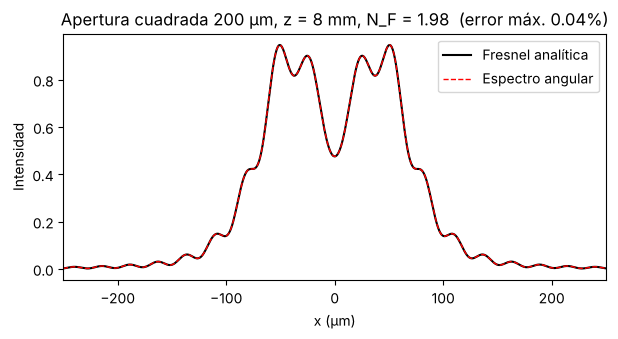
\includegraphics[width=0.85\textwidth]{b_apertura_cuadrada_fresnel.png}
\caption[Validación: apertura cuadrada]{Perfil de intensidad de una apertura cuadrada de
\SI{200}{\micro m} a \SI{8}{mm}: solución analítica de Fresnel y espectro angular.}
\label{fig:val-cuadrada}
\end{figure}

\begin{figure}[htb]
\centering
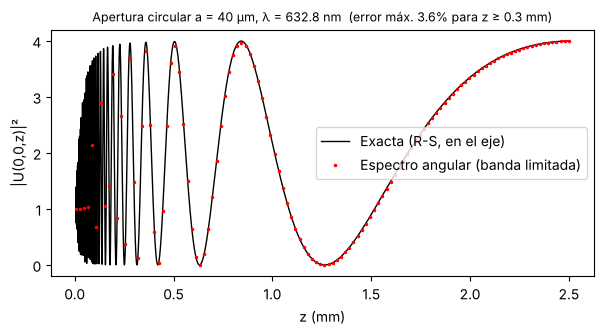
\includegraphics[width=0.85\textwidth]{a_apertura_circular.png}
\caption[Validación: apertura circular]{Intensidad en el eje de una apertura circular. Para
$z<\SI{0.3}{mm}$ el borde escalonado de un círculo pixelado cambia la fase de la onda de
borde, y las oscilaciones rápidas dejan de coincidir; no es un error del propagador sino de
la representación del círculo.}
\label{fig:val-circular}
\end{figure}

\begin{figure}[htb]
\centering
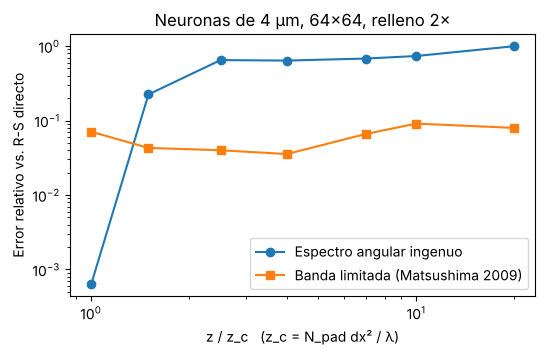
\includegraphics[width=0.7\textwidth]{c_aliasing_asm.png}
\caption[Validación: aliasing del espectro angular]{Error frente a la integral de
Rayleigh--Sommerfeld directa en función de $z/z_c$. El método ingenuo es exacto en $z=z_c$,
pero su error sube al 22--99\,\% en cuanto $z>z_c$; con límite de banda el error se mantiene
por debajo del 10\,\%. La comparación empieza en $z=z_c$ porque la suma directa sólo está
bien muestreada para $z\gtrsim z_c/2$, el régimen complementario.}
\label{fig:val-aliasing}
\end{figure}

\noindent El error residual del método de banda limitada (unos pocos por ciento) corresponde a
la luz que realmente sale de la ventana; la suma directa la cuenta y el propagador la
descarta. Para la red, cuyas capas son finitas, esa luz se perdería de todas formas.

% =====================================================================
\chapter{Resultados}\label{cap:resultados}
% =====================================================================

Todas las simulaciones usan el código del repositorio del proyecto \parencite{repo2026},
escrito en PyTorch \parencite{paszke2019} con el propagador de banda limitada del
\cref{cap:numerico}. Los dígitos provienen de la base MNIST \parencite{lecun1998}. Las
decisiones que el artículo no especifica se resumen en \cref{tab:decisiones}
(\cref{ap:implementacion}).

\section{Reproducción de la Fig.~6 del artículo}\label{sec:fig6}

Se entrenó la red reducida ($80\times80$ neuronas, 5 capas, 10 clases) en las configuraciones
de \cref{tab:casos}, con \num{10000} imágenes de entrenamiento, 500 de prueba, Adam con tasa
de aprendizaje \num{e-3} y 20 épocas. Cada caso tarda unos \SI{2.5}{min} en un procesador de
cuatro núcleos. \Cref{tab:fig6} compara las precisiones con las del artículo y \cref{fig:fig6b}
sitúa los casos respecto a la curva \eqref{eq:dmin}.

\begin{table}[htbp]
\centering
\caption[Reproducción de la Fig.~6(c) del artículo]{Precisión de prueba de la red
reducida ($80\times80$) en los casos de la Fig.~6(c) de \textcite{chen2021}.}
\label{tab:fig6}
\begin{tabular}{@{}lccccc@{}}
\toprule
Caso & $d_f$ ($\lambda$) & $D$ ($\lambda$) & $D/\Dmin$ & Artículo (\%) & Este trabajo (\%)\\
\midrule
1 & 0.53 & 15 & 1.01 & 90.0 & \textbf{89.8}\\
2 & 6 & $5.7\times10^3$ & 0.99 & 91.0 & \textbf{89.0}\\
3 (valor de la gráfica) & 6 & $2.4\times10^4$ & 4.18 & 91.2 & 84.8\\
3 (valor de la tabla) & 6 & $2.4\times10^3$ & 0.42 & 91.2 & \textbf{91.2}\\
4 & 12 & 15 & \num{6.5e-4} & ``$\sim$0.1'' & 14.4\\
\bottomrule
\end{tabular}
\end{table}

\begin{figure}[htbp]
\centering
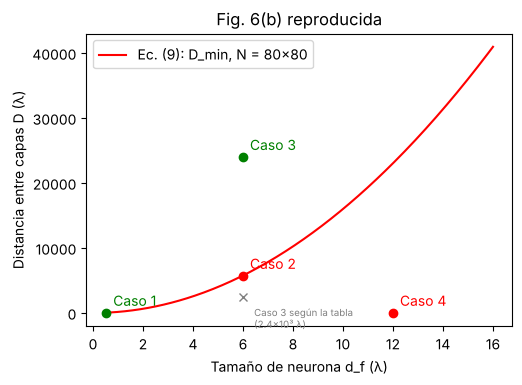
\includegraphics[width=0.62\textwidth]{e_fig6b_curva.png}
\caption[Curva de conectividad y casos de prueba]{Reproducción de la Fig.~6(b) de
\textcite{chen2021}: curva $\Dmin(d_f)$ de \cref{eq:dmin} para $\sqrt N=80$ y los cuatro
casos. Se marcan los dos valores del caso~3 que aparecen en el artículo.}
\label{fig:fig6b}
\end{figure}

\begin{figure}[htbp]
\centering
\begin{subfigure}{0.45\textwidth}\centering
  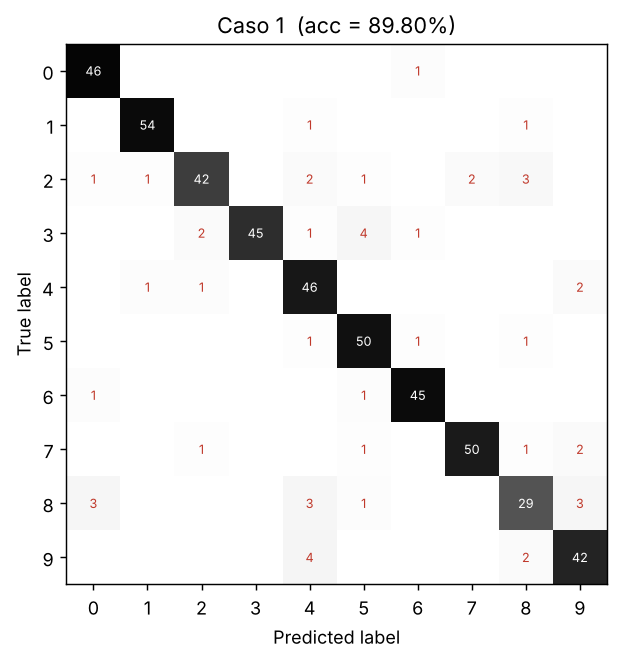
\includegraphics[width=\textwidth]{confusion_caso1.png}\caption{Caso 1}\end{subfigure}\hfill
\begin{subfigure}{0.45\textwidth}\centering
  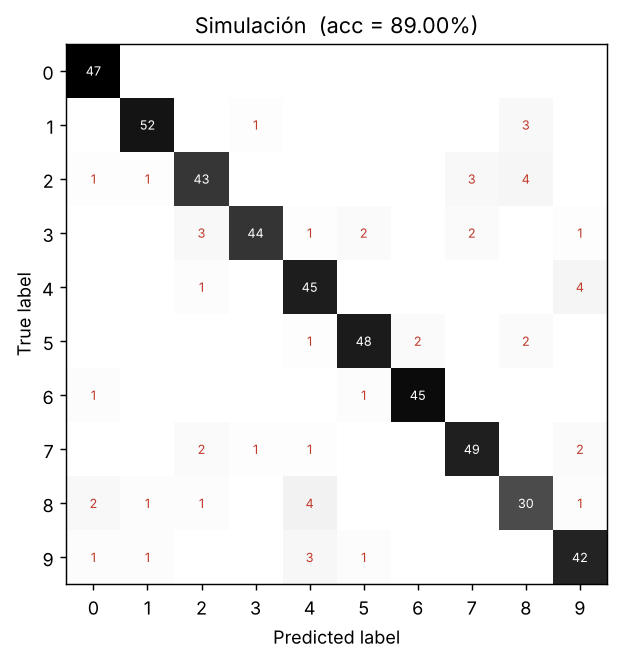
\includegraphics[width=\textwidth]{confusion_caso2.png}\caption{Caso 2}\end{subfigure}\\[4pt]
\begin{subfigure}{0.45\textwidth}\centering
  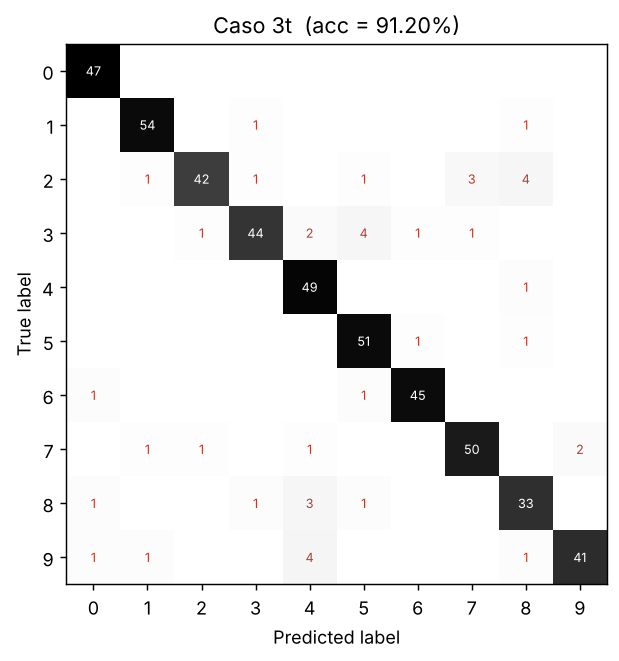
\includegraphics[width=\textwidth]{confusion_caso3_tabla.png}\caption{Caso 3 (valor de la tabla)}\end{subfigure}\hfill
\begin{subfigure}{0.45\textwidth}\centering
  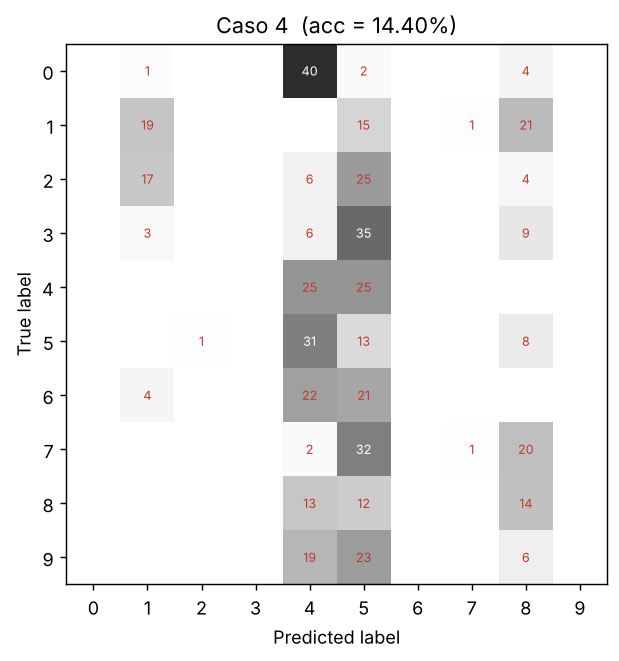
\includegraphics[width=\textwidth]{confusion_caso4.png}\caption{Caso 4}\end{subfigure}
\caption[Matrices de confusión de los casos de la Fig.~6]{Matrices de confusión sobre las
500 imágenes de prueba, equivalentes a las Figs.~6(d)--(g) del artículo. En el caso~4 las
predicciones se concentran en pocas columnas, como en la Fig.~6(g) original.}
\label{fig:confusiones}
\end{figure}

Los casos~1 y~2 se reproducen con una diferencia de 0.2 y 2 puntos porcentuales. El caso~4,
con neuronas grandes y capas muy próximas, no aprende: con $\varphi_{\max}=\ang{2.39}$ y
$D=15\lambda$, la luz se desplaza lateralmente $R=D\tan\varphi_{\max}\approx0.6\lambda$, menos de una
neurona. Cada capa sólo cambia la fase local, y una máscara de solo fase no modifica la
intensidad local; la distribución de intensidad en la salida es prácticamente la de la
entrada, sin importar cómo se entrenen las fases.

\FloatBarrier
\section{Inconsistencias en el artículo}\label{sec:inconsistencias}

\begin{enumerate}
  \item \textbf{El caso~3.} Con la distancia de la gráfica ($2.4\times10^4\lambda$, encima de la
  curva) se obtiene \SI{84.8}{\percent}; con la de la tabla ($2.4\times10^3\lambda$, debajo de la
  curva) se obtiene \SI{91.2}{\percent}, que coincide exactamente con el valor que reporta el
  artículo. Lo más probable es que la tabla sea la correcta y el punto de la gráfica esté mal
  colocado. En ese caso, el propio artículo contiene una configuración ``no totalmente
  conectada'' ($D=0.42\,\Dmin$) que funciona tan bien como las conectadas, lo que
  contradice la lectura de \eqref{eq:dmin} como condición necesaria.
  \item \textbf{El caso~4.} Una precisión de ``$\sim$\SI{0.1}{\percent}'' es imposible: el azar con
  10 clases da \SI{10}{\percent}. La matriz de confusión del artículo corresponde a una precisión
  de ese orden, así que el valor debe leerse como la fracción $0.1$. Aquí se obtiene
  \SI{14.4}{\percent}.
  \item \textbf{Alejar las capas no es gratis.} Con $D=4.18\,\Dmin$ la precisión baja de 89 a
  \SI{84.8}{\percent}. Como las capas son finitas, gran parte de la luz difractada cae fuera de
  la capa siguiente y se pierde; el artículo no toma en cuenta este efecto.
\end{enumerate}

\section{Barrido de la distancia entre capas}\label{sec:barrido}

El artículo valida su criterio con cuatro puntos. Para ver dónde se pierde realmente la
conectividad, se barrió $D/\Dmin$ de $10^{-3}$ a 3 para tres tamaños de neurona, con 20 épocas
por punto (\cref{fig:barrido,tab:barrido}).

\begin{figure}[htbp]
\centering
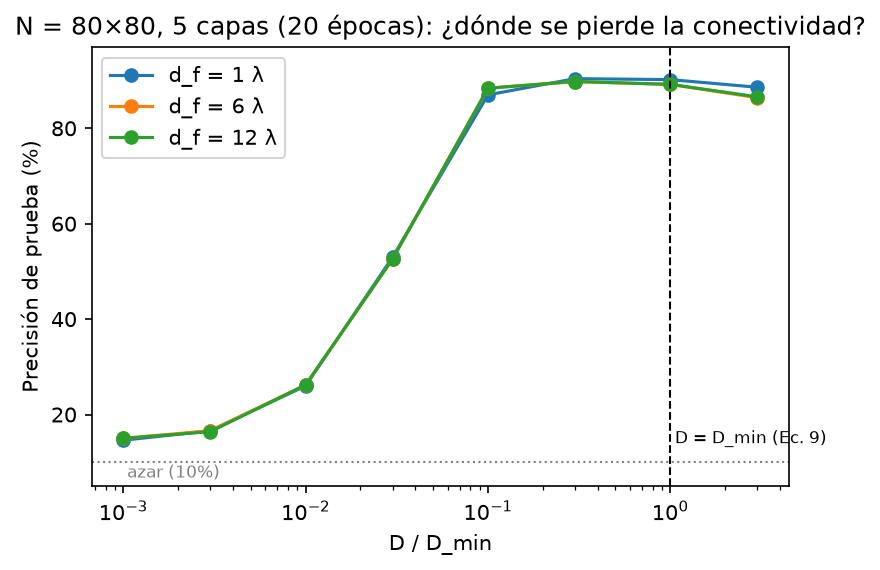
\includegraphics[width=0.72\textwidth]{sweep.png}
\caption[Barrido de conectividad]{Precisión de prueba en función de $D/\Dmin$ para
$d_f=1\lambda$, $6\lambda$ y $12\lambda$ ($\sqrt N=80$, 5 capas, 20 épocas). Las curvas coinciden y
la transición ocurre entre $0.03$ y $0.1\,\Dmin$, no en $D=\Dmin$.}
\label{fig:barrido}
\end{figure}

\begin{table}[htbp]
\centering
\caption{Precisión de prueba (\%) del barrido de conectividad (5 capas, 20 épocas).}
\label{tab:barrido}
\begin{tabular}{@{}lcccccccc@{}}
\toprule
$D/\Dmin$ & 0.001 & 0.003 & 0.01 & 0.03 & 0.1 & 0.3 & 1 & 3\\
\midrule
$d_f=1\lambda$  & 14.6 & 16.6 & 26.0 & 53.0 & 87.0 & 90.4 & 90.2 & 88.6\\
$d_f=6\lambda$  & 15.0 & 16.6 & 26.2 & 52.6 & 88.4 & 89.8 & 89.2 & 86.4\\
$d_f=12\lambda$ & 15.0 & 16.4 & 26.2 & 52.6 & 88.4 & 89.8 & 89.2 & 86.6\\
\bottomrule
\end{tabular}
\end{table}

\begin{resultado}{Conclusiones del barrido}
\begin{enumerate}
  \item \textbf{$D/\Dmin$ es la variable correcta.} Las tres curvas coinciden. Para $6\lambda$ y
  $12\lambda$ los resultados son prácticamente \emph{idénticos}, como predice \cref{prop:fresnel}: ambos
  sistemas tienen el mismo número de Fresnel por neurona y son ópticamente equivalentes. Con
  $d_f=1\lambda$, fuera del régimen paraxial, la diferencia sigue siendo menor a un punto
  en la zona de transición y alcanza hasta \num{2.2}~puntos en $D=3\,\Dmin$.
  \item \textbf{El criterio es suficiente pero unas diez veces más estricto de lo necesario.}
  Con $D=0.1\,\Dmin$ ya se alcanza el \SI{88.4}{\percent} (para $6\lambda$ y $12\lambda$), a sólo
  \num{1.4}~puntos del máximo en $0.3\,\Dmin$ (\SI{89.8}{\percent}).
  \item \textbf{Pasarse del criterio empeora.} En $D=3\,\Dmin$ la precisión baja a
  \SIrange{86.4}{88.6}{\percent} por la luz que escapa fuera de los bordes de las capas.
\end{enumerate}
\end{resultado}

Una explicación física del punto~2 es que la conectividad se \emph{acumula}: la red tiene
$L+1=6$ propagaciones y, aunque una sola no conecte bordes opuestos, la luz puede atravesar la
abertura transversal en varios saltos sucesivos. Si los radios de difracción se sumaran de
forma lineal bastaría $D\approx\Dmin/(L+1)=\Dmin/6\approx0.17\,\Dmin$; la transición observada
ocurre ligeramente antes (entre $0.03$ y $0.1\,\Dmin$).

Para comprobar esta hipótesis de \emph{conectividad acumulada}, se repitió el barrido fijando
$d_f=6\lambda$ y variando el número de capas difractivas $L\in\{1,3,5,8\}$ con 20 épocas por
punto (\cref{fig:barrido-capas,tab:barrido-capas}).

\begin{figure}[htbp]
\centering
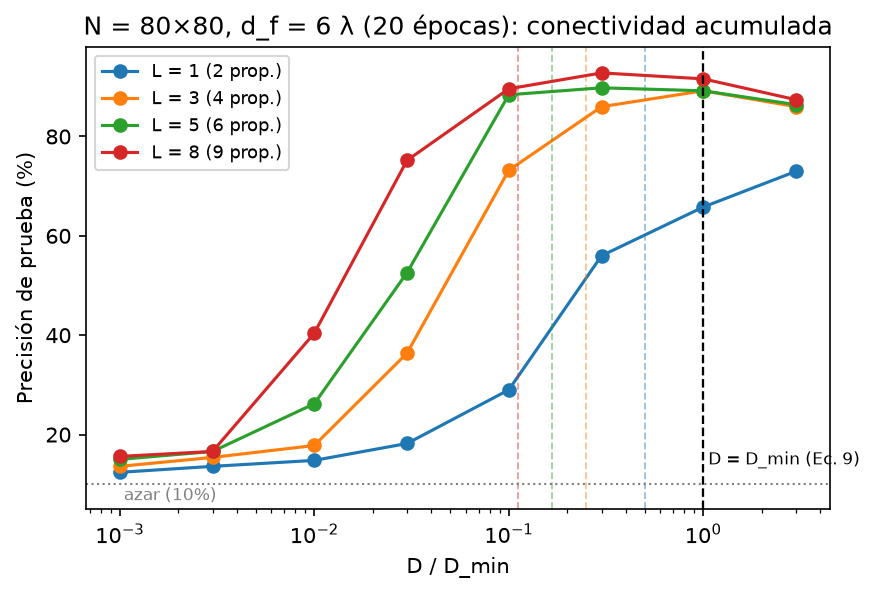
\includegraphics[width=0.72\textwidth]{sweep_layers.png}
\caption[Barrido de conectividad por número de capas]{Precisión de prueba en función de
$D/\Dmin$ para $L\in\{1,3,5,8\}$ capas ($d_f=6\lambda$, $\sqrt N=80$, 20 épocas). Las líneas
verticales punteadas de cada color indican el umbral estimado $D/\Dmin=1/(L+1)$. Al aumentar el
número de capas, la curva de transición se desplaza sistemáticamente hacia distancias menores.}
\label{fig:barrido-capas}
\end{figure}

\begin{table}[htbp]
\centering
\caption{Precisión de prueba (\%) variando el número de capas $L$ ($d_f=6\lambda$, 20 épocas).}
\label{tab:barrido-capas}
\begin{tabular}{@{}lccccccccc@{}}
\toprule
Capas $L$ ($L+1$ prop.) & $\frac{1}{L+1}$ & 0.001 & 0.003 & 0.01 & 0.03 & 0.1 & 0.3 & 1 & 3\\
\midrule
$L=1$ (2 prop.) & 0.500 & 12.4 & 13.6 & 14.8 & 18.2 & 29.0 & 56.0 & 65.8 & 73.0\\
$L=3$ (4 prop.) & 0.250 & 13.6 & 15.4 & 17.8 & 36.4 & 73.2 & 86.0 & 89.2 & 86.0\\
$L=5$ (6 prop.) & 0.167 & 15.0 & 16.6 & 26.2 & 52.6 & 88.4 & 89.8 & 89.2 & 86.4\\
$L=8$ (9 prop.) & 0.111 & 15.6 & 16.6 & 40.4 & 75.2 & 89.6 & 92.8 & 91.6 & 87.4\\
\bottomrule
\end{tabular}
\end{table}

Los resultados confirman directamente la hipótesis y revelan dos efectos acoplados:
\begin{enumerate}
  \item \textbf{Desplazamiento sistemático del umbral con $L+1$.} Al incrementar el número de
  etapas de propagación, el codo de transición se recorre hacia la izquierda en la escala
  logarítmica de $D/\Dmin$: en $D=0.03\,\Dmin$, la precisión crece monótonamente de
  \SI{18.2}{\percent} ($L=1$) a \SI{36.4}{\percent} ($L=3$), \SI{52.6}{\percent} ($L=5$) y
  \SI{75.2}{\percent} ($L=8$). De igual modo, en $D=0.1\,\Dmin$, $L=1$ apenas logra
  \SI{29.0}{\percent} y $L=3$ llega a \SI{73.2}{\percent}, mientras que $L=5$ y $L=8$ ya entran
  en la meseta de alta precisión (\SI{88.4}{\percent} y \SI{89.6}{\percent}). Esto concuerda con
  la escala $D/\Dmin\sim 1/(L+1)$, pues las máscaras sucesivas pueden dirigir haces difractados en
  ángulo acumulado a través de las $L+1$ propagaciones.
  \item \textbf{Capacidad expresiva frente a conectividad.} Con una sola capa ($L=1$), aun en
  $D=\Dmin$ y $D=3\,\Dmin$ (donde un único salto ya conecta toda la abertura), la precisión se
  estanca en \SI{65.8}{\percent} y \SI{73.0}{\percent}. Ello demuestra que, además de permitir la
  mezcla espacial por difracción, apilar varias máscaras de fase ($L\ge 3$) es indispensable para
  aumentar los grados de libertad de la transformación óptica, alcanzando \SI{92.8}{\percent} con
  $L=8$ en $D=0.3\,\Dmin$.
\end{enumerate}

\FloatBarrier
\section{Funcionamiento de la red entrenada}\label{sec:funcionamiento}

\Cref{fig:fases,fig:ejemplos,fig:corte} muestran la red del caso~2 una vez entrenada.

\begin{figure}[htbp]
\centering
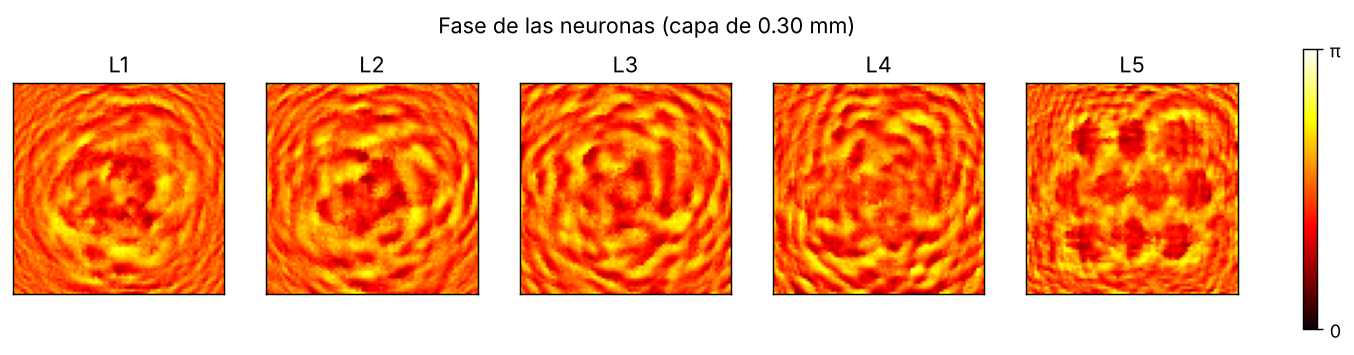
\includegraphics[width=\textwidth]{fases.png}
\caption[Fases entrenadas]{Fases de las cinco capas entrenadas (caso~2), equivalentes a la
Fig.~1(b) del artículo.}
\label{fig:fases}
\end{figure}

\begin{figure}[htbp]
\centering
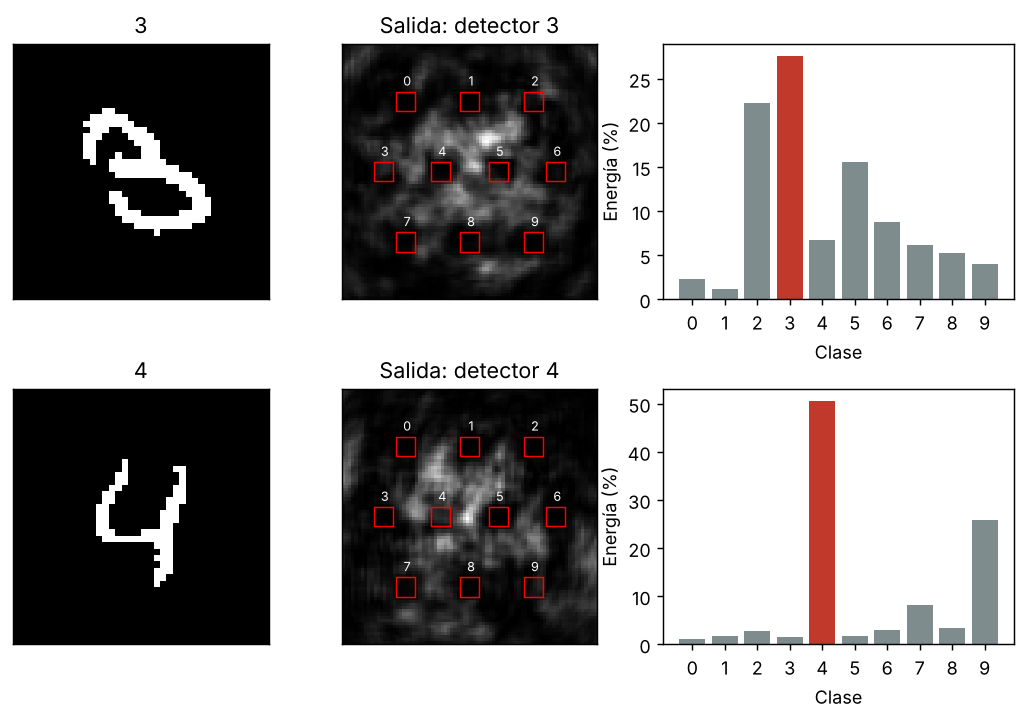
\includegraphics[width=0.9\textwidth]{fig3_ejemplos.png}
\caption[Ejemplos de clasificación]{Objeto de entrada, intensidad en el plano de salida con
los detectores y distribución de energía entre detectores, como en la Fig.~3 del artículo.}
\label{fig:ejemplos}
\end{figure}

\begin{figure}[htbp]
\centering
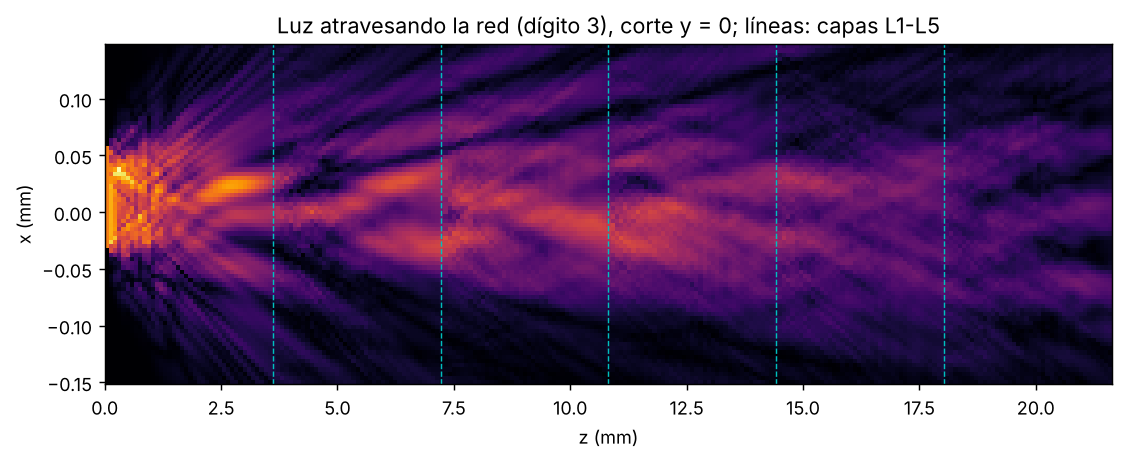
\includegraphics[width=\textwidth]{corte_xz.png}
\caption[Corte longitudinal de la intensidad]{Intensidad en el plano $y=0$ a lo largo de
todo el sistema para un dígito 3. Las líneas punteadas son las capas. La luz se redistribuye
capa a capa hasta concentrarse en el detector correcto.}
\label{fig:corte}
\end{figure}

En las máscaras de fase entrenadas (\cref{fig:fases}) se distingue una clara división funcional
entre capas. Las primeras cuatro capas (\texttt{L1}--\texttt{L4}) presentan patrones
cuasi-concéntricos de anillos y rejillas curvas de frecuencia espacial creciente: recuerdan a
placas zonales de Fresnel deformadas que reciben el haz modulado en amplitud por el dígito de
entrada y desvían sus componentes de Fourier hacia distintas regiones transversales de la
abertura de \SI{0.30}{mm}. En contraste, la última máscara (\texttt{L5}) organiza sus fases en
un arreglo explícito de diez sub-aberturas focalizadoras dispuestas exactamente en la
geometría 3--4--3 de los detectores (\cref{fig:fases}, derecha): actúa como una matriz de
microlentes difractivas que concentra la energía ya clasificada en cada caja receptora
(\cref{fig:ejemplos}).

El corte longitudinal $x\text{--}z$ en el plano $y=0$ (\cref{fig:corte}) ilustra esta evolución
espacial para un dígito~3. En $z=0$, la luz atraviesa únicamente los trazos binarios del
dígito en la región central ($|x|\lesssim\SI{0.06}{mm}$) y se expande por difracción en forma
de abanico hasta alcanzar la primera máscara (\texttt{L1}, $z\approx\SI{3.6}{mm}$). A lo largo
de \texttt{L1}--\texttt{L4} ($z\in[3.6,\,14.4]\,\si{mm}$), la modulación de fase redirige el
frente de onda para contener la energía dentro de la abertura finita y canalizarla mediante
interferencia constructiva en trayectorias oblicuas bien definidas; finalmente, después de
\texttt{L5} ($z\approx\SI{18.0}{mm}$), la intensidad converge selectivamente sobre el plano de
salida ($z\approx\SI{21.6}{mm}$) en la coordenada transversal del detector correspondiente.

\FloatBarrier
\section{Tolerancias de fabricación}\label{sec:fabricacion}

El artículo reporta \SI{91.57}{\percent} en simulación y \SI{84}{\percent} en el experimento. Para
estimar qué imperfecciones explican esa diferencia, se evaluó la red del caso~2 (neuronas de
\SI{3.8}{\micro m}) \emph{sin reentrenar} bajo cuatro tipos de error (\cref{fig:fabricacion}).

\begin{figure}[htbp]
\centering
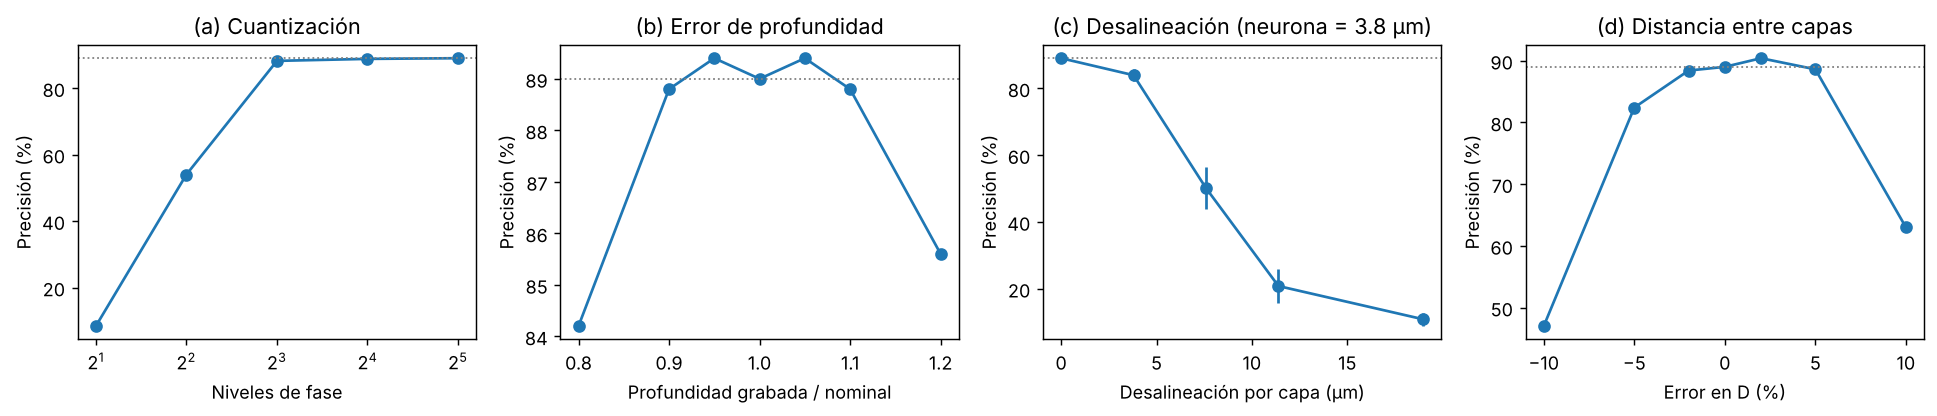
\includegraphics[width=0.90\textwidth]{fabricacion.png}
\caption[Tolerancias de fabricación]{Precisión de la red del caso~2 ante (a) cuantización
de la fase, (b) error en la profundidad grabada, (c) desalineación lateral aleatoria de cada
capa y (d) error en la distancia entre capas. La línea punteada es la red ideal
(\SI{89.0}{\percent}).}
\label{fig:fabricacion}
\end{figure}

\begin{table}[htbp]
\centering
\caption{Precisión (\%) de la red del caso~2 bajo errores de fabricación.}
\label{tab:fabricacion}
\begin{tabular}{@{}llcccccc@{}}
\toprule
\multirow{2}{*}{(a) Cuantización} & niveles & 2 & 4 & 8 & 16 & 32 & \\
 & precisión & 8.4 & 54.0 & 88.2 & 88.8 & 89.0 & \\
\midrule
\multirow{2}{*}{(b) Profundidad} & real/nominal & 0.8 & 0.9 & 0.95 & 1.05 & 1.1 & 1.2\\
 & precisión & 84.2 & 88.8 & 89.4 & 89.4 & 88.8 & 85.6\\
\midrule
\multirow{2}{*}{(c) Desalineación} & neuronas (\si{\micro m}) & 1 (3.8) & 2 (7.6) & 3 (11.4) & 5 (19.0) & & \\
 & precisión & 83.9 & 50.1 & 20.8 & 10.8 & & \\
\midrule
\multirow{2}{*}{(d) Distancia} & error en $D$ & $-10\%$ & $-5\%$ & $-2\%$ & $+2\%$ & $+5\%$ & $+10\%$\\
 & precisión & 47.0 & 82.4 & 88.4 & 90.4 & 88.6 & 63.0\\
\bottomrule
\end{tabular}
\end{table}

La malla numérica tiene una muestra por neurona, por lo que sólo pueden simularse
desplazamientos laterales de un número entero de neuronas; en cada evaluación, cada capa se
desplaza exactamente $k$ neuronas en una dirección aleatoria independiente (5 repeticiones).

\begin{resultado}{Conclusiones de fabricación}
\begin{itemize}
  \item Hacen falta al menos \textbf{8 niveles de fase} (3 pasos de litografía): con 4 niveles la
  precisión cae al \SI{54}{\percent}.
  \item La tolerancia más crítica es la \textbf{alineación lateral}: desplazar cada capa una
  sola neurona (\SI{3.8}{\micro m}) baja la precisión al \SI{83.9}{\percent}, prácticamente la
  cifra experimental del artículo, y dos neuronas la reducen al \SI{50}{\percent}.
  \item Un error de $\pm\SI{10}{\percent}$ en la profundidad apenas afecta, y la distancia entre
  capas tolera $\pm\SI{5}{\percent}$.
\end{itemize}
\end{resultado}

\FloatBarrier
\section{Sistema completo de \texorpdfstring{$1000\times1000$}{1000x1000} neuronas}\label{sec:sistema-completo}

El sistema completo del artículo consiste en 5 capas difractivas de $1000\times1000$ neuronas
($d_f=\SI{4}{\micro m}$, abertura $w=\SI{4}{mm}$, separación $D=\SI{50}{mm}\approx\Dmin$),
11 clases (dígitos 0--9 y la clase adicional~X para dígitos tapados o alterados),
\num{80000} imágenes de entrenamiento (\num{55000} de MNIST y \num{25000} modificadas) y
\num{11000} imágenes de prueba (\num{10000} y \num{1000}, respectivamente). Dado el costo de
propagar arreglos complejos rellenados de $2000\times2000$ puntos (\cref{sec:costo}), la red se
entrenó en la RTX~5060~Ti (\cref{sec:hardware}) con tamaño de lote óptimo \texttt{--bs 24}
(\num{3334} iteraciones de Adam por época) durante 6 épocas completas (\num{20004} pasos de
gradiente).

La evolución por época (\cref{tab:full-hist}) muestra una rápida convergencia inicial
(\SI{79.11}{\percent} tras la época~1 y \SI{88.32}{\percent} en la época~3) seguida de una
aproximación asintótica a la meseta en la época~6, donde la precisión de prueba alcanza
\textbf{\SI{90.63}{\percent}} en un tiempo total de \SI{10537}{s} (\SI{2}{h} \SI{56}{min}).
\Cref{tab:full} resume el desempeño frente a \textcite{chen2021}: la diferencia respecto al
\SI{91.57}{\percent} del artículo es menor a un punto porcentual (\num{0.94}~puntos porcentuales), pese a
entrenar 6 épocas en lugar de 20 y emplear nuestra propia generación sintética de la clase~X.

\begin{table}[!htbp]
\centering
\caption{Convergencia por época del sistema completo de $1000\times1000$ neuronas (\texttt{--bs 24}, RTX~5060~Ti).}
\label{tab:full-hist}
\begin{tabular}{@{}ccccc@{}}
\toprule
Época & Pérdida (train) & Precisión train (\%) & Precisión test (\%) & Tiempo acumulado\\
\midrule
1 & 1.2509 & 64.12 & 79.11 & \SI{30.0}{min}\\
2 & 0.6865 & 83.61 & 85.96 & \SI{60.3}{min}\\
3 & 0.5451 & 87.45 & 88.32 & \SI{89.5}{min}\\
4 & 0.4808 & 89.08 & 89.49 & \SI{118.2}{min}\\
5 & 0.4421 & 90.11 & 89.95 & \SI{146.9}{min}\\
\textbf{6} & \textbf{0.4156} & \textbf{90.79} & \textbf{90.63} & \textbf{\SI{175.6}{min} (\SI{2.93}{h})}\\
\bottomrule
\end{tabular}
\end{table}

\begin{table}[!htbp]
\centering
\small
\caption[Resultados del sistema completo de $1000\times1000$ neuronas]{Comparación del sistema completo ($1000\times1000$ neuronas, 11 clases) frente a \textcite{chen2021}.}
\label{tab:full}
\begin{tabularx}{\textwidth}{@{}>{\raggedright\arraybackslash}X>{\centering\arraybackslash}p{4.3cm}>{\centering\arraybackslash}p{4.3cm}@{}}
\toprule
Métrica & Artículo (20 épocas) & Este trabajo (6 épocas)\\
\midrule
Precisión total (11 clases, \num{11000} imgs.) & \SI{91.57}{\percent} & \textbf{\SI{90.63}{\percent}}\\
Dígitos sin cambio (0--9, \num{10000} imgs.) & --- & \textbf{\SI{90.24}{\percent}}\\
Clase X (tapados o alterados, \num{1000} imgs.) & --- & \textbf{\SI{94.50}{\percent}}\\
Tiempo de entrenamiento & $\approx\SI{20}{h}$ ($\approx\SI{1}{h}$/época, GTX~1080) & \SI{2.93}{h} (\SI{29.3}{min}/época, RTX~5060~Ti)\\
\bottomrule
\end{tabularx}
\end{table}

\Cref{fig:full-confusion,fig:full-fases,fig:full-ejemplos,fig:full-seises,fig:full-onda,fig:full-corte}
muestran el comportamiento óptico del modelo de $1000\times1000$ evaluado con
\texttt{05\_evaluate.py}. En la matriz de confusión (\cref{fig:full-confusion}), todas las
clases concentran su diagonal con alta pureza —destacando el dígito~1 (\num{1100} aciertos) y
la clase~X (\SI{94.50}{\percent})—, y la mayor fuente de error residual corresponde a dígitos
difíciles (como el~2 o el~5) rechazados hacia la clase~X. Las máscaras de fase
(\cref{fig:full-fases}) exhiben rejillas difractivas finas en \texttt{L1}--\texttt{L3} y
concentran progresivamente once microlentes difractivas en \texttt{L4}--\texttt{L5} siguiendo
exactamente la disposición 3--2--2--2--2 de los 11 detectores del plano de salida.

Los ejemplos individuales confirman la selectividad espacial del clasificador: un 3 o un 4
íntegros enfocan la mayor parte de la energía en su detector nominal, mientras que sus
versiones alterada o tapada redirigen el \SIrange{50}{73}{\percent} de la energía detectada
hacia la caja~X (\cref{fig:full-ejemplos}); cuatro realizaciones distintas del dígito~6
concentran de manera consistente su máximo en el detector~6 (\cref{fig:full-seises}); y una
onda plana uniforme sin dígito (\cref{fig:full-onda}) es enviada casi por completo al detector~X
($\approx\SI{89}{\percent}$), evidenciando que la red aprende a tratar cualquier patrón no
reconocible como objeto fuera de clase. El corte longitudinal $x\text{--}z$
(\cref{fig:full-corte}) muestra la expansión del frente de onda a lo largo de los
\SI{300}{mm} totales del tren óptico y su canalización hacia los haces desviados de salida.

\begin{figure}[htbp]
\centering
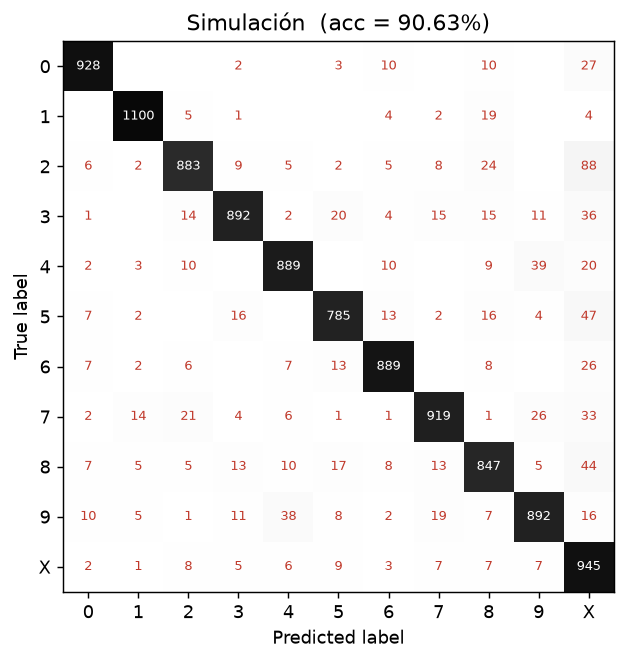
\includegraphics[width=0.62\textwidth]{full_confusion.png}
\caption[Matriz de confusión del sistema completo]{Matriz de confusión del sistema completo de
$1000\times1000$ neuronas sobre \num{11000} imágenes de prueba (precisión global del
\SI{90.63}{\percent}).}
\label{fig:full-confusion}
\end{figure}

\begin{figure}[htbp]
\centering
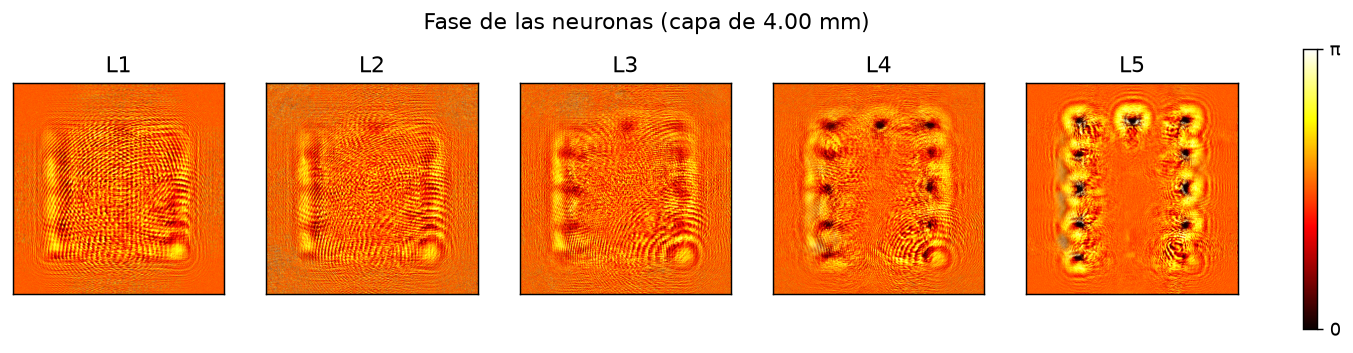
\includegraphics[width=\textwidth]{full_fases.png}
\caption[Fases entrenadas del sistema completo]{Máscaras de fase \texttt{L1}--\texttt{L5}
($4.00\times 4.00\,\si{mm}$, $1000\times1000$ neuronas) del sistema completo. En \texttt{L5}
se distinguen las 11 microlentes correspondientes al arreglo de detectores de la Fig.~3(b) del
artículo.}
\label{fig:full-fases}
\end{figure}

\begin{figure}[htbp]
\centering
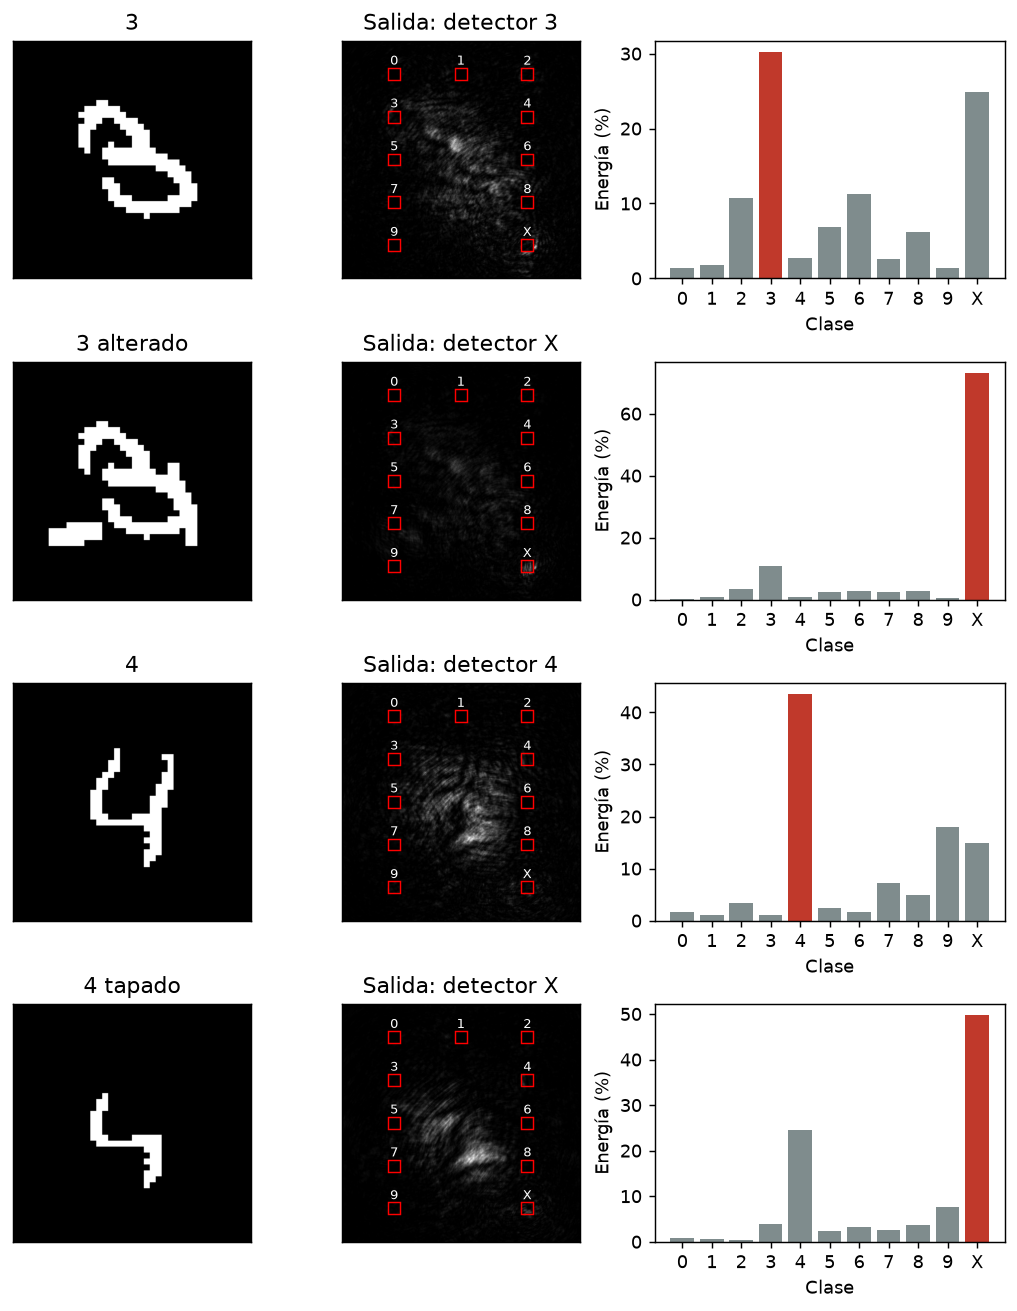
\includegraphics[width=0.88\textwidth]{full_fig3_ejemplos.png}
\caption[Ejemplos de clasificación con clase X]{Respuesta del sistema completo para un 3
intacto, un 3 alterado, un 4 intacto y un 4 tapado (equivalente a la Fig.~3 del artículo).}
\label{fig:full-ejemplos}
\end{figure}

\begin{figure}[htbp]
\centering
\begin{subfigure}{0.49\textwidth}\centering
  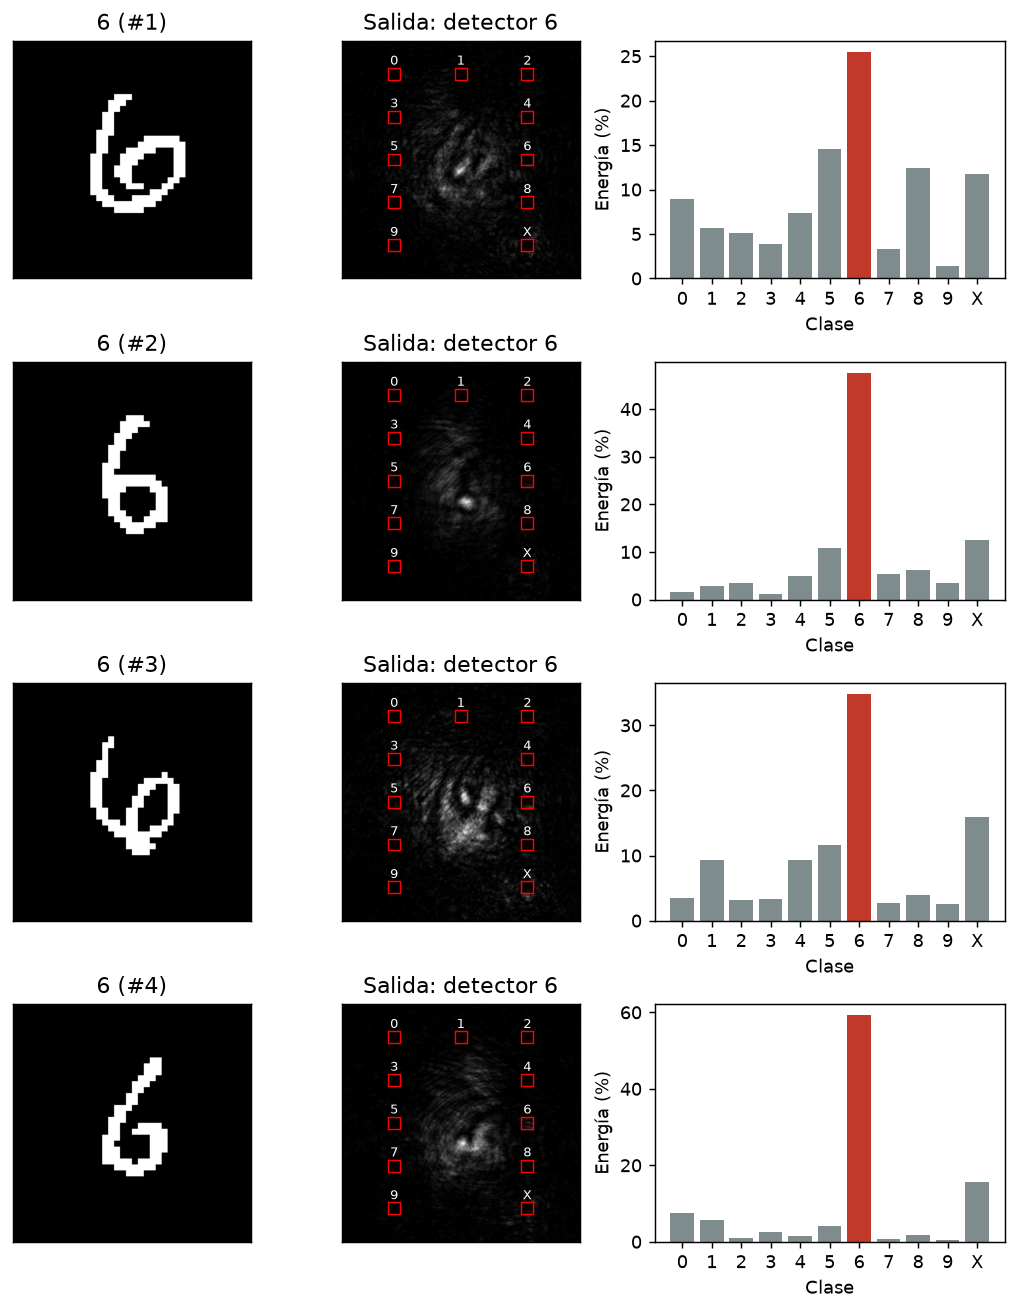
\includegraphics[width=\textwidth]{full_fig4_seises.png}
  \caption{Cuatro dígitos 6 distintos (cf.\ Fig.~4 del artículo)}
  \label{fig:full-seises}
\end{subfigure}\hfill
\begin{subfigure}{0.49\textwidth}\centering
  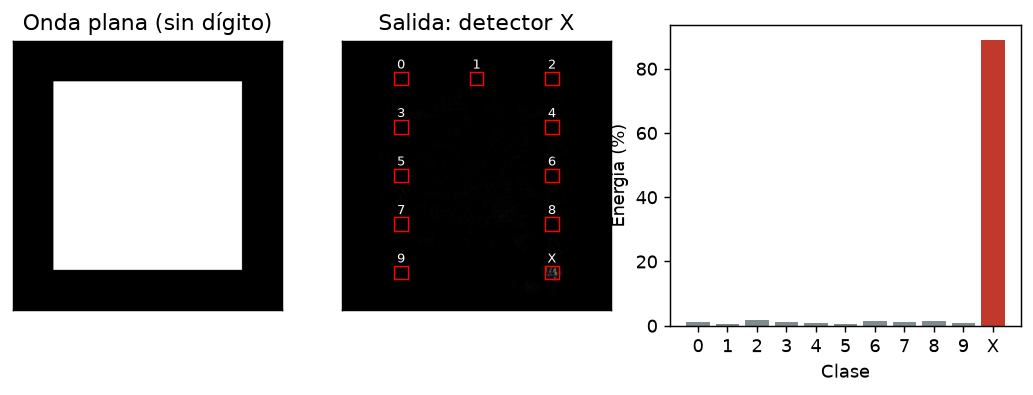
\includegraphics[width=\textwidth]{full_fig5_onda_plana.png}
  \caption{Onda plana sin dígito (cf.\ Fig.~5 del artículo)}
  \label{fig:full-onda}
\end{subfigure}
\caption[Generalización intra-clase y rechazo de onda plana]{(a) Cuatro variantes manuscritas
del dígito~6 enfocan en el detector~6; (b) una onda plana sin objeto se dirige al detector~X.}
\label{fig:full-seises-onda}
\end{figure}

\begin{figure}[htbp]
\centering
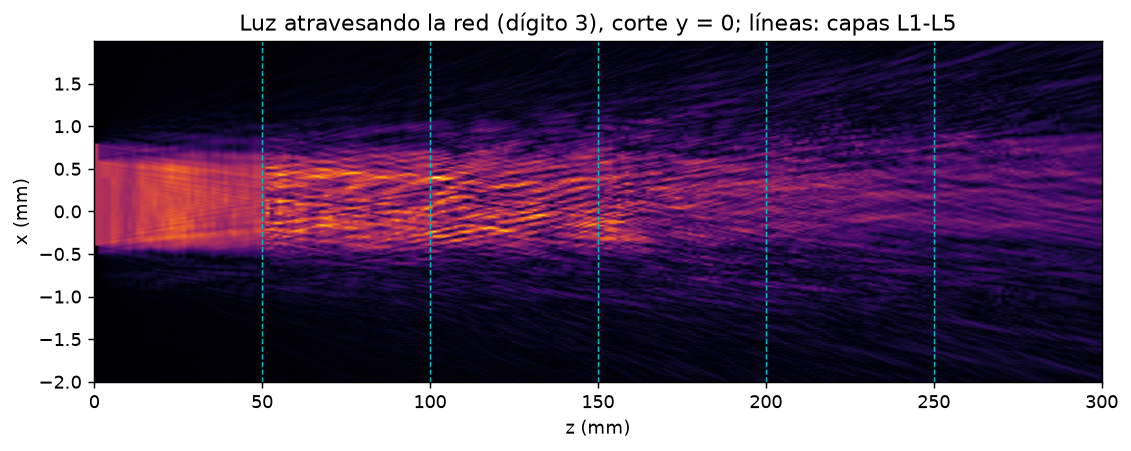
\includegraphics[width=\textwidth]{full_corte_xz.png}
\caption[Corte longitudinal del sistema completo]{Corte longitudinal $x\text{--}z$ en $y=0$
a lo largo de los \SI{300}{mm} del sistema completo para un dígito~3 (líneas punteadas en
$z=50, 100, 150, 200, 250\,\si{mm}$).}
\label{fig:full-corte}
\end{figure}

Finalmente, se repitió el análisis de tolerancias de fabricación sobre el modelo de
$1000\times1000$ en \num{2000} imágenes de prueba (\cref{fig:full-fabricacion}, línea base
ideal \SI{91.35}{\percent}). Mientras que la cuantización a 8 niveles sigue bastando con
holgura (\SI{91.05}{\percent}, e incluso 4 niveles conservan \SI{87.50}{\percent}) y los
errores de profundidad de $\pm\SI{10}{\percent}$ mantienen \SIrange{89.65}{91.70}{\percent}, la
sensibilidad a la distancia axial $D$ se vuelve mucho más severa que en el caso~2 de
$80\times80$: una desviación de $\pm\SI{2}{\percent}$ en $D=\SI{50}{mm}$ ($\pm\SI{1}{mm}$) hace
caer la precisión a \SIrange{12.05}{15.05}{\percent}. La razón cuantitativa es la siguiente.

\paragraph{Tolerancia axial.} Un error $\Delta D$ en la distancia multiplica el espectro de
cada capa por $H(u,v;\Delta D)\approx e^{\jj k\Delta D}\,e^{-\jj\pi\lambda\Delta D(u^2+v^2)}$
(\cref{eq:fresnel-tf}). En el borde de la banda controlable, $u=1/(2d_f)$, el error de fase
es $\pi\lambda\Delta D/(4d_f^2)$. Exigir que no supere $\pi/2$ da
\begin{equation}
  \Delta D\le\frac{2d_f^2}{\lambda}
  \qquad\Longrightarrow\qquad
  \frac{\Delta D}{D}\le\frac{2d_f^2}{\lambda D}=2N_{F,n}\approx\frac{1}{\sqrt N}\,\frac{\Dmin}{D},
  \label{eq:tol-axial}
\end{equation}
donde se usó \eqref{eq:dmin-paraxial}. La tolerancia relativa decrece como $1/\sqrt N$:
\begin{center}
\begin{tabular}{@{}lccc@{}}
\toprule
Sistema & $2d_f^2/\lambda$ & $D$ & $\Delta D/D$ tolerable\\
\midrule
Caso 2 ($\sqrt N=80$) & \SI{45.6}{\micro m} & \SI{3.6}{mm} & \SI{1.3}{\percent}\\
Completo ($\sqrt N=1000$) & \SI{50.6}{\micro m} & \SI{50}{mm} & \SI{0.10}{\percent}\\
\bottomrule
\end{tabular}
\end{center}
Esto explica por qué el caso~2 tolera $\pm\SI{2}{\percent}$ mientras que en el sistema completo
el mismo error relativo, unas 20 veces la tolerancia, lleva la precisión al nivel del azar:
\textbf{redes más grandes, separadas cerca de $\Dmin$, son proporcionalmente más sensibles a la
distancia entre capas.}

En cuanto a la alineación lateral, desplazar cada capa una sola neurona (\SI{4}{\micro m})
reduce la precisión del sistema completo a \SI{81.4 \pm 3.5}{\percent}; dos neuronas, a
\SI{38.4 \pm 19.5}{\percent}; y tres o más la llevan al nivel del azar
(\SIrange{8.7}{12.8}{\percent}). Al igual que en el caso~2, una neurona de desalineación basta
para explicar la diferencia entre la precisión simulada y la experimental del artículo.

\begin{figure}[htbp]
\centering
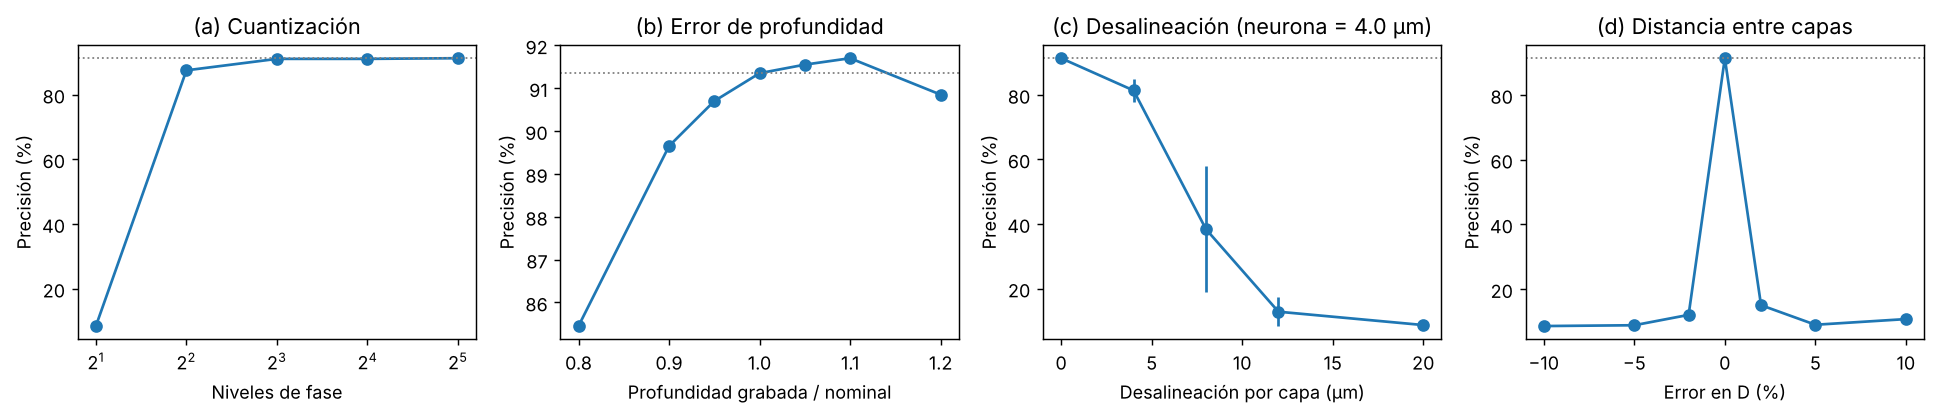
\includegraphics[width=0.88\textwidth]{full_fabricacion.png}
\caption[Tolerancias de fabricación del sistema completo]{Sensibilidad del sistema de
$1000\times1000$ neuronas (precisión ideal de \SI{91.35}{\percent} en \num{2000} imágenes) ante
(a) cuantización, (b) error de profundidad, (c) desalineación lateral y (d) variación porcentual
de $D=\SI{50}{mm}$.}
\label{fig:full-fabricacion}
\end{figure}

\FloatBarrier
\subsection{Eficiencia de detección}\label{sec:eficiencia}

La pérdida \eqref{eq:perdida} usa la energía \emph{relativa} entre detectores, así que no
premia que la luz llegue a ellos. Midiendo la eficiencia
$\eta=\sum_kE_k/\iint|Y^{\text{sal}}|^2$, sólo el \SI{1.1}{\percent} de la luz de salida del
sistema completo cae en los detectores (\SI{1.6}{\percent} en el caso~2), menos que la
fracción del plano que ocupan (\SI{2.75}{\percent} y \SI{5.6}{\percent}). La red clasifica bien,
pero en un experimento con ruido de fondo esa eficiencia sería un problema.

Añadiendo a la pérdida un término $w\,(1-\eta)$ se obtiene un compromiso entre precisión y
eficiencia (caso~2, 20 épocas):
\begin{center}
\begin{tabular}{@{}lcccc@{}}
\toprule
Peso $w$ & 0 & 1 & 3 & 10\\
\midrule
Precisión (\%) & 89.0 & 88.6 & 85.8 & 64.6\\
Eficiencia $\eta$ (\%) & 1.6 & 2.2 & 18.6 & 89.4\\
\bottomrule
\end{tabular}
\end{center}
Con $w=3$ la eficiencia se multiplica por 11 a cambio de 3 puntos de precisión.

% =====================================================================
\chapter{Discusión y conclusiones}\label{cap:conclusiones}
% =====================================================================

\section{Conclusiones}

\begin{enumerate}
  \item El modelo de \textcite{chen2021} se deduce por completo de la teoría escalar de la
  difracción: la función de transferencia del espacio libre sale de la ecuación de Helmholtz
  (\cref{sec:espectro-angular}), y el semiángulo $\varphi_{\max}=\arcsin[\lambda/(2d_f)]$ es el
  ángulo asociado a la frecuencia de Nyquist de la malla de neuronas, no al primer cero de
  difracción de una neurona (\cref{sec:neurona}).
  \item El sistema opera en campo cercano ($N_F\approx126$) y fuera de la validez de la
  aproximación de Fresnel para las componentes más inclinadas, por lo que es necesario usar
  la función de transferencia exacta (\cref{sec:fresnel}).
  \item El gradiente del entrenamiento es el término de interferencia entre la onda que viaja
  hacia adelante y una onda de error que viaja hacia atrás con la función de transferencia
  conjugada; la deducción coincide con la diferenciación automática a precisión de máquina
  (\cref{sec:gradiente}).
  \item El criterio de conectividad del artículo es idéntico a la condición de muestreo del
  espectro angular de banda limitada (\cref{prop:identidad}) y, en el régimen paraxial,
  equivale a una condición sobre el número de Fresnel de una neurona (\cref{prop:fresnel}).
  \item La simulación reproduce las precisiones del artículo (\cref{tab:fig6}), confirma la
  hipótesis de conectividad acumulada mediante el barrido de capas $L\in\{1,3,5,8\}$
  (\cref{sec:barrido}), detecta dos inconsistencias en su Fig.~6 (\cref{sec:inconsistencias}) y
  reproduce el sistema completo de $1000\times1000$ neuronas y 11 clases en GPU con
  \SI{90.63}{\percent} de precisión en prueba (\cref{sec:sistema-completo}).
  \item La alineación lateral de las capas —una sola neurona de desplazamiento baja la precisión a
  $\approx\SI{84}{\percent}$ en el caso~2 y $\approx\SI{81}{\percent}$ en el sistema completo— y
  la separación axial $D$, cuya tolerancia relativa escala como $1/\sqrt N$ (\SI{0.10}{\percent}
  de $D$ en el sistema completo), son las tolerancias de fabricación más exigentes y explican la
  brecha entre simulación y experimento (\cref{sec:fabricacion,sec:sistema-completo}).
\end{enumerate}

\section{Limitaciones}

\begin{itemize}
  \item \textbf{Aproximación escalar.} Es razonable para $d_f\approx6\lambda$, pero no para el
  caso~1 ($d_f=0.53\lambda$), donde los efectos vectoriales y de acoplamiento entre neuronas
  vecinas pueden ser importantes \parencite[sec.~3.2]{goodman2005}.
  \item \textbf{Capas delgadas.} Cada capa se modela como una máscara infinitamente delgada; un
  relieve de \SI{0.7}{\micro m} junto a neuronas de \SI{4}{\micro m} no es estrictamente delgado.
  \item \textbf{Elementos del artículo no especificados.} La forma de los detectores, la
  normalización de la pérdida, la codificación de la entrada y el conjunto de dígitos
  alterados se tuvieron que elegir (\cref{tab:decisiones}), y pueden explicar parte de las
  diferencias.
  \item \textbf{Sin experimento.} Todos los resultados son numéricos.
\end{itemize}

\section{Trabajo futuro}

\begin{itemize}
  \item \textbf{Entrenamiento robusto ante imperfecciones:} incorporar aleatoriamente durante el
  entrenamiento desplazamientos laterales, variaciones en la distancia $D$ y cuantización de
  fase (\emph{error-aware training}) para cerrar la brecha entre simulación y experimento.
  \item \textbf{Modelado electromagnético vectorial:} emplear métodos FDTD o RCWA en arreglos
  con $d_f\lesssim\lambda$, donde el acoplamiento cercano y el relieve físico finito dejan de
  ser despreciables.
  \item \textbf{Fabricación experimental e iluminación policromática:} evaluar el desempeño
  de las máscaras cuantizadas en sílice fundida ante desalineaciones multigrado y múltiples
  longitudes de onda.
\end{itemize}

\section{Valoración final}

Este proyecto muestra que un problema moderno de cómputo óptico se explica por completo con las
herramientas fundamentales de la óptica ondulatoria: la ecuación de Helmholtz, el espectro
angular de ondas planas, el teorema de muestreo de Shannon--Nyquist y la escala fijada por el
número de Fresnel. Lejos de ser una caja negra numérica, cada regla de diseño y cada límite de
resolución de una D\textsuperscript{2}NN tienen una raíz física transparente: desde la
identidad exacta entre el criterio de conectividad y el límite de banda del propagador, hasta
el papel de la interferencia holográfica en el cálculo de su gradiente. En cuanto a la promesa
de la computación óptica, las D\textsuperscript{2}NN resultan especialmente atractivas para
tareas de procesamiento visual y filtrado pasivo de baja latencia —donde la luz clasifica o
transforma un frente de onda sin consumo energético adicional durante la inferencia—, aunque
su escalamiento práctico frente a arquitecturas electrónicas seguirá condicionado por la
linealidad de la propagación libre, la tolerancia de alineación sub-micrométrica y el cuello de
botella optoelectrónico en las etapas de entrada y detección.


\printbibliography[title={Referencias}]

\appendix
% =====================================================================
\chapter{Deducción de la integral de Rayleigh--Sommerfeld}\label{ap:rs}
% =====================================================================

Este apéndice deduce \eqref{eq:rs}--\eqref{eq:h-rs} siguiendo a
\textcite[secs.~3.3--3.5]{goodman2005}.

\section{Teorema integral de Helmholtz y Kirchhoff}

Sean $U$ y $G$ dos funciones que satisfacen la ecuación de Helmholtz \eqref{eq:helmholtz}
dentro de un volumen $V$ limitado por una superficie $S$. El teorema de Green afirma que
\begin{equation}
  \iiint_V\bigl(G\nabla^2U-U\nabla^2G\bigr)\dd V
  =\oiint_S\Bigl(G\frac{\partial U}{\partial n}-U\frac{\partial G}{\partial n}\Bigr)\dd S,
  \label{eq:green}
\end{equation}
con $\partial/\partial n$ la derivada en la dirección de la normal exterior. Como
$\nabla^2U=-k^2U$ y $\nabla^2G=-k^2G$, el integrando de la izquierda se anula. Si se elige
$G=e^{\jj kr_{01}}/r_{01}$, una onda esférica que sale del punto de observación $P_0$, hay que
excluir de $V$ una esfera pequeña alrededor de $P_0$, donde $G$ es singular. Al hacer tender su
radio a cero, esa esfera contribuye con $4\pi U(P_0)$, y se obtiene el \emph{teorema integral de
Helmholtz y Kirchhoff}:
\begin{equation}
  U(P_0)=\frac{1}{4\pi}\oiint_S\Bigl(G\frac{\partial U}{\partial n}-U\frac{\partial G}{\partial n}\Bigr)\dd S .
  \label{eq:hk}
\end{equation}

\section{Elección de la superficie y de la función de Green}

Tomamos como $S$ el plano $z=0$ cerrado por una semiesfera de radio $R\to\infty$ en $z>0$. Si el
campo satisface la condición de radiación de Sommerfeld,
$\lim_{R\to\infty}R\,(\partial U/\partial n-\jj kU)=0$, la contribución de la semiesfera se anula
y sólo queda el plano.

Para no tener que conocer a la vez $U$ y $\partial U/\partial n$ en el plano, Sommerfeld propuso
usar la función de Green
\begin{equation}
  G_-=\frac{e^{\jj kr_{01}}}{r_{01}}-\frac{e^{\jj k\tilde r_{01}}}{\tilde r_{01}},
  \label{eq:green-imagen}
\end{equation}
donde $\tilde r_{01}$ es la distancia desde el punto imagen $\tilde P_0=(x_0,y_0,-z_0)$. En el
plano $z=0$ ambas distancias son iguales, así que $G_-=0$ y \eqref{eq:hk} se reduce a
\begin{equation}
  U(P_0)=-\frac{1}{4\pi}\iint_{z=0}U\,\frac{\partial G_-}{\partial n}\dd S .
  \label{eq:rs-paso}
\end{equation}

\section{Cálculo de la derivada normal}

En el plano la normal exterior apunta hacia $-z$, de modo que $\partial/\partial n=-\partial/\partial z_1$.
Para el primer término de \eqref{eq:green-imagen}, con
$r_{01}^2=(x_1-x_0)^2+(y_1-y_0)^2+(z_1-z_0)^2$,
\[
  \frac{\partial r_{01}}{\partial z_1}\Big|_{z_1=0}=-\frac{z_0}{r},\qquad
  \frac{\partial}{\partial r}\Bigl(\frac{e^{\jj kr}}{r}\Bigr)=\Bigl(\jj k-\frac1r\Bigr)\frac{e^{\jj kr}}{r},
\]
y por lo tanto $\partial G_1/\partial n=(\jj k-1/r)(e^{\jj kr}/r)(z_0/r)$. Para el término imagen,
$\partial\tilde r_{01}/\partial z_1=+z_0/r$ y la derivada tiene el signo opuesto, pero aparece
restando en $G_-$. Ambas contribuciones se suman:
\begin{equation}
  \frac{\partial G_-}{\partial n}=2\,\frac{z_0}{r}\Bigl(\jj k-\frac1r\Bigr)\frac{e^{\jj kr}}{r}.
  \label{eq:dgdn}
\end{equation}
Sustituyendo en \eqref{eq:rs-paso}, con $z\equiv z_0$,
\begin{equation}
  U(x_0,y_0,z)=\frac{1}{2\pi}\iint U(x_1,y_1,0)\,\frac{z}{r}\Bigl(\frac1r-\jj k\Bigr)\frac{e^{\jj kr}}{r}\dd x_1\dd y_1,
\end{equation}
que es \eqref{eq:rs} con la respuesta al impulso \eqref{eq:h-rs}.

\section{Ejemplo resuelto: campo en el eje de una apertura circular}\label{sec:circular}

Este resultado sirve como referencia exacta en \cref{tab:validacion}. Una apertura
circular de radio $a$ se ilumina con una onda plana unitaria. En el eje ($x_0=y_0=0$), con
coordenadas polares $\rho$ en la apertura, $r^2=z^2+\rho^2$:
\[
  U(0,0,z)=\frac{1}{2\pi}\int_0^{2\pi}\!\!\int_0^a\frac{z}{r^2}\Bigl(\frac1r-\jj k\Bigr)e^{\jj kr}\,\rho\dd\rho\dd\phi
  =z\int_0^a\Bigl(\frac1r-\jj k\Bigr)\frac{e^{\jj kr}}{r^2}\,\rho\dd\rho .
\]
Como $r\dd r=\rho\dd\rho$, el cambio de variable de $\rho$ a $r$ (de $z$ a $R=\sqrt{z^2+a^2}$) da
\[
  U(0,0,z)=z\int_z^R\Bigl(\frac{1}{r^2}-\frac{\jj k}{r}\Bigr)e^{\jj kr}\dd r .
\]
El integrando es la derivada de $-e^{\jj kr}/r$; en efecto,
$\frac{\dd}{\dd r}\bigl(-e^{\jj kr}/r\bigr)=e^{\jj kr}/r^2-\jj k\,e^{\jj kr}/r$. Por lo tanto
\begin{equation}
  \boxed{\;U(0,0,z)=z\Bigl[-\frac{e^{\jj kr}}{r}\Bigr]_z^R=e^{\jj kz}-\frac{z}{R}\,e^{\jj kR}.\;}
  \label{eq:circular}
\end{equation}
El primer término es la onda incidente y el segundo, una onda que parece salir del borde de la
apertura. Su interferencia produce las oscilaciones de \cref{fig:val-circular}: la
intensidad en el eje se anula cada vez que la diferencia de camino $R-z$ es un múltiplo entero
de $\lambda$ (si $z\gg a$ y $z/R\approx1$), lo que equivale a que la apertura contenga un número
par de zonas de Fresnel \parencite[sec.~10.3]{hecht2017}.

% =====================================================================
\chapter{Detalles de implementación}\label{ap:implementacion}
% =====================================================================

\section{Algoritmo de entrenamiento}

\begin{algorithm}[htb]
\caption{Entrenamiento de la D\textsuperscript{2}NN}\label{alg:entrenamiento}
\begin{algorithmic}[1]
\Require imágenes $\{(X_b,y_b)\}$, parámetros $\theta^1,\dots,\theta^L$, tasa $\eta=10^{-3}$
\State Calcular $H(u,v;D)$ en doble precisión, con el límite de banda \eqref{eq:flim}
\For{época $=1,\dots,E$}\Comment{$E=20$ en Fig.~6 y barridos; $E=6$ en el sistema completo}
  \For{cada lote $(X,y)$}
    \State $Y\gets$ codificar $X$ como amplitud (binaria) en el plano de entrada
    \State $Y\gets\mathcal{P}_D\{Y\}$
    \For{$l=1,\dots,L$}
       \State $\Phi^l\gets\pi\,\sigma(\theta^l)$;\quad $Y\gets\mathcal{P}_D\{Y\circ e^{\jj\Phi^l}\}$
       \Comment{\cref{eq:capa-a-capa}}
    \EndFor
    \State $E_k\gets\sum_{i\in\text{det}_k}|Y_i|^2$;\quad $\mathcal{L}\gets$ \cref{eq:perdida}
    \State $\partial\mathcal{L}/\partial\theta^l\gets$ retropropagación (\cref{sec:gradiente})
    \State $\theta^l\gets\mathrm{Adam}(\theta^l,\partial\mathcal{L}/\partial\theta^l,\eta)$
  \EndFor
\EndFor
\Ensure fases $\Phi^l=\pi\sigma(\theta^l)$ y alturas $\Delta h^l=\lambda\Phi^l/(2\pi\Delta n)$
\end{algorithmic}
\end{algorithm}

\section{Decisiones no especificadas en el artículo}

\Cref{tab:decisiones} resume las elecciones de implementación en aspectos que \textcite{chen2021} no especifican.

\begin{table}[!htbp]
\centering
\caption{Decisiones de la reproducción en aspectos que \textcite{chen2021} no especifican.}
\label{tab:decisiones}
\begin{tabularx}{\textwidth}{@{}>{\raggedright}p{4.2cm}X@{}}
\toprule
Aspecto & Elección en este trabajo\\
\midrule
Propagador & Espectro angular de banda limitada \parencite{matsushima2009}, relleno al doble, $H$ en doble precisión\\
Tamaño finito de las capas & El campo se recorta a $w\times w$ después de cada propagación\\
Distancias entrada--L1 y L5--salida & Iguales a $D$\\
Codificación de la entrada & Dígito MNIST escalado (vecino más cercano) al \SI{70}{\percent} del lado y binarizado, como máscara de cromo\\
Detectores & Cuadrados del \SI{5}{\percent} del lado con el arreglo de la Fig.~3(b) del artículo (11 clases); arreglo 3--4--3 del \SI{8}{\percent} para la Fig.~6\\
Pérdida & Entropía cruzada con softmax sobre la energía relativa, temperatura $T=10$ (\cref{eq:perdida})\\
Inicialización & $\theta\sim\mathcal N(0,0.1^2)$, es decir $\Phi\approx\pi/2$\\
Dígitos cambiados (clase X) & No publicados. Se generan: \SI{50}{\percent} tapados (un rectángulo borra entre el 25 y el \SI{65}{\percent} del trazo) y \SI{50}{\percent} alterados (2 o 3 trazos adicionales)\\
Caso 3 de la Fig.~6 & Se simulan los dos valores de $D$ que aparecen en el artículo\\
\bottomrule
\end{tabularx}
\end{table}

\FloatBarrier
\section{Reproducibilidad}

El código, los resultados y este documento están en el repositorio del proyecto
\parencite{repo2026}. Los pasos para reproducir cada resultado son:
\begin{lstlisting}[language=bash,numbers=none,basicstyle=\ttfamily\scriptsize]
python -m pytest -q tests                      # pruebas unitarias
python scripts/01_validate_optics.py            # capítulo 5
python scripts/02_fig6_cases.py                 # sección 6.1
python scripts/03_connectivity_sweep.py --device cuda --epochs 20
python scripts/03_connectivity_sweep.py --device cuda --epochs 20 --layers 1 3 5 8
python scripts/07_check_gradient.py             # tabla 3.2
python scripts/05_evaluate.py results/02_fig6/fig6_case2/model.pt
python scripts/06_fabrication_errors.py results/02_fig6/fig6_case2/model.pt
python scripts/04_train_full.py --epochs 6 --bs 24 --max-minutes 185  # sistema completo (GPU)
python scripts/05_evaluate.py results/04_full/paper_full/model.pt --bs 24
python scripts/06_fabrication_errors.py results/04_full/paper_full/model.pt --bs 24
\end{lstlisting}

\section{Equipo de cómputo y rendimiento}\label{sec:hardware}

Las simulaciones aceleradas por GPU se ejecutaron en una estación de trabajo equipada con una
tarjeta gráfica \textbf{NVIDIA GeForce RTX 5060 Ti} de \SI{16}{GiB} de VRAM (arquitectura
Blackwell, capacidad de cómputo \texttt{sm\_120}, controlador \texttt{615.71.09}) utilizando
\texttt{PyTorch 2.10.0+cu128} con soporte nativo para CUDA~12.8.

Para seleccionar el tamaño de lote óptimo en el modelo completo ($N = 1000\times 1000$
neuronas, malla rellenada de $2000\times 2000$ puntos complejos en precisión simple
\texttt{complex64} y 5 capas difractivas sin \emph{gradient checkpointing}), se ejecutó el
banco de pruebas \texttt{scripts/benchmark.py} (\cref{tab:benchmark}).

\begin{table}[htb]
\centering
\caption{Rendimiento y consumo de VRAM por tamaño de lote en la RTX 5060 Ti (\SI{16}{GiB}) para el modelo de $1000\times 1000$ neuronas.}
\label{tab:benchmark}
\begin{tabular}{@{}cccccc@{}}
\toprule
Lote & ms/iteración & ms/imagen & Época (\num{80000} img.) & 20 épocas & VRAM pico (\si{GiB})\\
\midrule
16 & 332.6 & 20.78 & \SI{27.7}{min} & \SI{9.24}{h} & 4.77\\
\textbf{24} & \textbf{487.6} & \textbf{20.32} & \textbf{\SI{27.1}{min}} & \textbf{\SI{9.03}{h}} & \textbf{7.03}\\
32 & 660.2 & 20.63 & \SI{27.5}{min} & \SI{9.17}{h} & 9.30\\
48 & \multicolumn{5}{c}{Excede la VRAM disponible (\emph{CUDA out of memory})}\\
64 & \multicolumn{5}{c}{Excede la VRAM disponible (\emph{CUDA out of memory})}\\
\bottomrule
\end{tabular}
\end{table}

El tamaño de lote \texttt{--bs 24} ofrece el mayor rendimiento efectivo
(\SI{20.32}{ms} por imagen, \SI{487.6}{ms} por iteración y \SI{27.1}{min} por época completa de
\num{80000} imágenes) consumiendo \SI{7.03}{GiB} de VRAM pico, menos de la mitad de la memoria
disponible en la GPU. Con \texttt{--bs 32} el tiempo por imagen se satura ligeramente
(\SI{20.63}{ms} por imagen, \SI{9.30}{GiB}), mientras que a partir de \texttt{--bs 48} las FFT
complejas de $2000\times 2000$ sobrepasan los \SI{15.56}{GiB} útiles de la tarjeta.

En la corrida final del sistema completo (\texttt{--epochs 6 --bs 24}), cada época completa
—incluyendo la evaluación sobre las \num{11000} imágenes de prueba y el guardado atómico del
punto de control— tomó en promedio \SI{29.3}{min}, completando las 6 épocas (\num{20004}
actualizaciones de Adam) en \SI{10537}{s} (\SI{2}{h} \SI{56}{min}) hasta alcanzar una
precisión de prueba de \SI{90.63}{\percent}.


\end{document}
